\documentclass[12pt]{iopart}
\usepackage{graphicx}% Include figure files

\bibliographystyle{PV}
\begin{document}
\title[]{Acoustically driven degradation in single crystalline Si solar cell}

\author{O Ya Olikh}

\address{Faculty of Physics, Taras Shevchenko National University of Kyiv, Kyiv 01601, Ukraine}
\ead{olikh@univ.kiev.ua}

\begin{abstract}
The experimental investigation of ultrasound influence on the silicon solar cell current-voltage characteristic has been carried out.
The experiments were carried out by  using  longitudinal and transverse ultrasound waves  in the temperature range from 290 to 340~K.
The investigation has revealed the acoustically driven reversible increment of an ideality factor and decrement of a carrier lifetime both in the space charge region and in the solar cell base, a photocurrent, an open--circuit voltage,  a fill factor, and a shunt resistance.
The models of coupled defect level recombination, Shockley--Read--Hall recombination, and dislocation--induced impedance were used to describe the processes in the space charge region,  in the solar cell base, and shunt resistance respectively.
The role of oxide precipitates in an recombination and in an acousto--defect interaction has been discussed.
It has been shown that the acoustically induced increase of carrier capture coefficient of point or extended defects is a reason of observed effects and qualitative model of ultrasound influence has been proposed.
\end{abstract}

%\pacs{73.30.+y, 43.35.Ty, 43.35.+d, 72.20.-i, 73.40.-c}
\noindent{Keywords: \it silicon, solar cells, ultrasound influence\/ }

%\maketitle

%\ioptwocol


\section{Introduction}

The silicon solar cells (SSC) are still dominant in the photovoltaic (PV) field due to their high efficiency, low selling price and process maturity.
Therefore, understanding the way of material properties modification is a top priority for  most of PV device manufacturers.
It is known, for example, the loss in the SSC efficiency is observed in consequence of
excess carrier injection by above-bandgap illumination or forward biasing \cite{LID:BothePP,LID:SchmidtJMR,LIDRev,LID:JAP2017II} (so--called light--induced degradation or LID),
high voltage stress \cite{PID:SEMSC,PID:PP,PID:2017} (potential--induced degradation or PID),
or radiation treatment \cite{Bhat,Karazhanov} (irradiation--induced degradation or IID).
Degradation reasons are processes in crystal defect sub-system under external influence.
It is may be a transformation of the boron-oxygen or copper-contained complex (for the LID case),
a decoration of stacking faults by sodium (PID case) or
a creation of radiation--induced recombination centers (IID case).
The partial or full SSC efficiency recovery is observed quite often during of subsequent annealing at an elevated temperature.

On the other hand, it has been shown experimentally that ultrasonic  waves (USWs) can be the effective instrument for defect engineering in silicon.
In particular, ultrasound is used
to affect a carrier diffusion length \cite{Ostapenko1999,Ostrovskii2001},
to vary a current in  p--n structures and Schottky diodes \cite{OlikhJAP,Olikh2011Sem,Davletova2009,Davletova2008,YOlikh2005,Olikh:Ultras},
to transform an impurity defect \cite{Korotchenkov1995,Ostapenko1995,Olikh2009Sem,UST:Medvid},
to change a spectrum  \cite{Zaver:2008} and density \cite{Mirsagatov} of surface states.
Frequently the crystal and device properties recover after stopping of ultrasound action at room temperature even \cite{Ostapenko1999,Ostrovskii2001,OlikhJAP,Korotchenkov1995}.

This article presents the result of experimentally investigation of the acoustic strain field influence on the electrical characteristic of the n$^+$--p SSC.
Ultrasound has been found to result the decrease of carriers lifetime and, accordingly, solar cell efficiency.
The USWs intensity did not exceed $0.5$~W/cm$^2$ and the full recovery of cell characteristics was observed after the stop of an acoustic wave propagation.
Dependencies of such sound induced degradation on USW type and intensity are presented.
%Features of such sound induced degradation are presented.
The findings are discussed by using models of coupled defect level recombination, Shockley--Read--Hall (SRH) recombination, and dislocation--induced impedance.
% \cite{CDLR:JAP1995,CDLR:JAP}.


\section{Experimental and calculation details}

The investigated solar cell was created on 2 inch p-type CZ-Si:B wafers with doping level of $1.4\times10^{15}$~cm$^{-3}$ and thickness of 300~$\mu$m.
The n$^+$ emitter with carrier concentration of about $10^{19}$~cm$^{-3}$ and thickness of 0.5~$\mu$m was formed by phosphorus implantation.
Then wafer surface was passivated by Al$_2$O$_3$ film and further capped by TiO$_x$ as antireflective coating.
Finally the aluminium front (metal grid) and rear (solid contact) electrodes were deposited by screen printing before rapid annealing.
The samples with area of $1.5$ to $2.1$~cm$^{2}$ used in our experiments were cut from the central part of the wafer.

The dark and illuminated forward current-voltage ($I$--$V$) characteristics of the samples both with and without ultrasound loading (USL)  were measured over a temperature range 290--340~K.
The sample temperature was controlled by differential copper-constantan thermocouple.
Some curves are shown in \Fref{figIV}.

The classical double-diode model of n$^+$--p SSC $I$--$V$ characteristics expressed in the following form:
\begin{eqnarray}
\label{eqIV}
\nonumber I(V,T)&=&-AJ_{ph}+\frac{qAn_id}{2\tau_{g}}\left\{\exp \left[\frac{q(V-IR_s)}{nkT}\right]-1\right\}\\
&&+\frac{qAn_i^2}{p_p}\sqrt{\frac{\mu_nkT}{\tau_n}}\left\{\exp \left[\frac{q(V-IR_s)}{kT}\right]-1\right\}+\frac{V-IR_s}{R_{sh}}\,,
\end{eqnarray}
where $A$ is the cell area,
$J_{ph}$ is the photocurrent density,
$n_i$ is the intrinsic carrier concentration,
$\tau_{g}$ is the carrier lifetime in the space charge region (SCR),
$d$ is the  SCR thickness:
\begin{equation}
\label{eqW}
    d(V,T)=\sqrt{\frac{2 \varepsilon \varepsilon_0(p_p+n_n)}{q p_p n_n}\left[\frac{E_g}{q}-\frac{kT}{q}\ln\left(\frac{N_vN_c}{p_pn_n}\right)-\frac{2kT}{q}-V\right]} \,,
\end{equation}
$\varepsilon$ is the permittivity (11.7 for Si),
$p_p$ and $n_n$ are the majority carrier concentration in the $p$-- and $n$--type regions,
$E_g$ is the semiconductor band gap,
$N_c$ and $N_v$ are the effective density of states in the conduction and valence bands;
$n$ is the ideality factor of the nonideal current components,
$R_s$ and $R_{sh}$ are the series and shunt resistances of the device,
$\mu_n$ and $\tau_n$ are the electron (minority carrier) mobility and lifetime outside SCR in the diode base.
The current-voltage  equation that models the solar cell by  an equivalent electrical circuit contains several parameters related to physical phenomena occurring in  the device.
It is commonly believed that $I_{01}=(qAn_i^2/n_n)\sqrt{\mu_nkT/\tau_n}$ is closely related to recombination in the quasi-neutral region, while $I_{0n}=(qAdn_i/2\tau_{g})$ reflects the overall recombination in the SCR.

\begin{figure}
\begin{center}
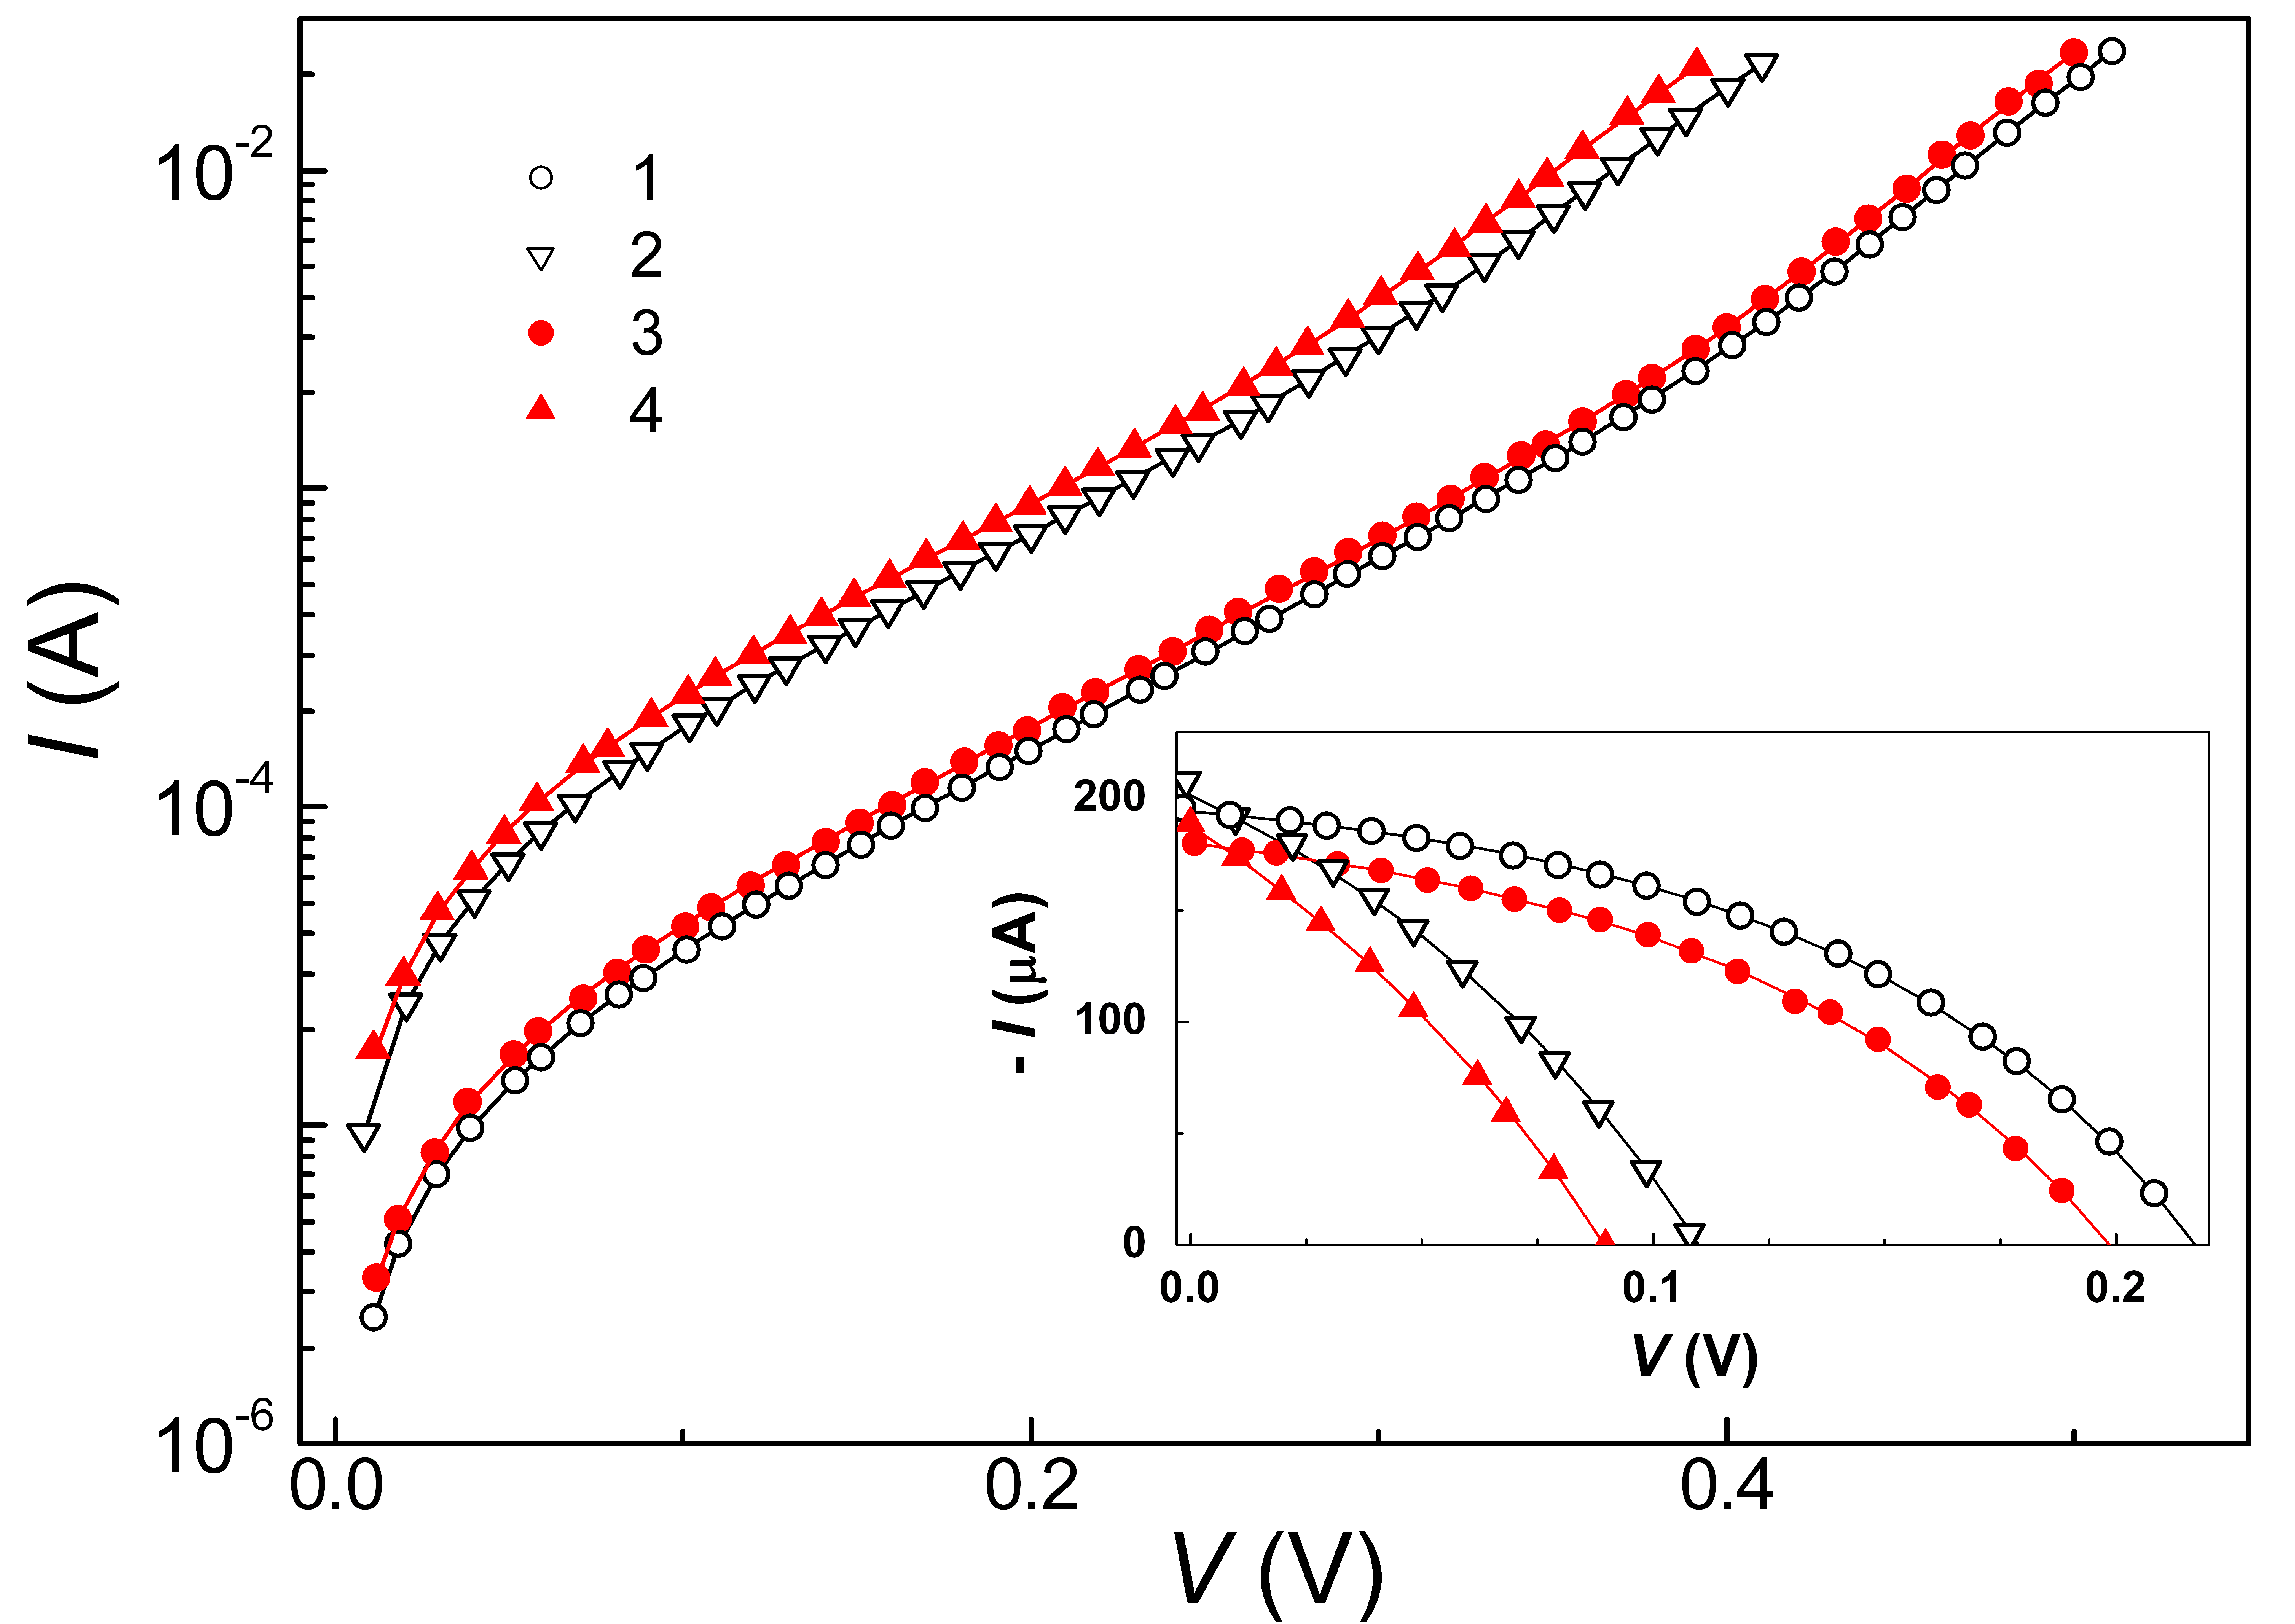
\includegraphics[width=7.5cm]{olikhFig1}%
\end{center}
\caption{\label{figIV}
SSC dark $I$--$V$ characteristics measured at 301~K (curves 1, 3) and 341~K (curves 2, 4)
with (2, 4) and without(1, 3) USL.
$W_{U\!S}=0.40$~W/cm$^2$.
Inset: Parts of illuminated $I$--$V$ characteristics in the voltage range from 0 to $V_{oc}$.
The lines are the fitted curves using Eq.~(\ref{eqIV}).
}%
\end{figure}

We used Eqs. (\ref{eqIV}) and (\ref{eqW}) to fit the experimental data and the $I_{ph}$ (for illuminated $I$--$V$ curves only), $\tau_g$, $\tau_n$, $n$, $R_{sh}$, and $R_s$ were taken as the  fittings parameters.
It was supposed that $n_i=1.64\times10^{15}\,T^{1.706}\exp(-E_g/2kT)$ \cite{ni:Green} and temperature dependencies of $E_g$ and $\mu_n$ followed Varshni and Caughey--Thomas equations \cite{Schroder2006,Markvart}
\begin{eqnarray}
\label{eqEg}
E_g(T) = 1.169 - 7.021\cdot10^{-4} T^2 /(T + 1108)\,,\\
\label{eqMu}
\mu_n(T) = \mu_{min}+\frac{\mu_0}{1+(p_p/N_{ref})^{\zeta}}\,.
\end{eqnarray}
%\begin{equation}
%\label{eqEg}
%E_g(T) = 1.169 - 7.021\cdot10^{-4} T^2 /(T + 1108)\,,
%\end{equation}
%and a Caughey--Thomas form \cite{Schroder2006,Markvart}
%\begin{equation}
%\label{eqMu}
%\mu_n(T) = \mu_{min}+\frac{\mu_0}{1+(p_p/N_{ref})^{\zeta}}\,.
%\end{equation}
The temperature dependence of the $\mu_{min}$, $\mu_0$, $N_{ref}$ and $\zeta$
%various parameters in Eq.~(\ref{eqMu})
has the form $P=P_0(T/300)^{\gamma}$ and parameters value are given in the \cite{Schroder2006}, Table~A8.2.
The fitting were done by using the differential evolution method \cite{DEWang} and extremely good fit to the experimental data was obtained --- see \Fref{figIV}.

The monochromatic light was used for SSC illumination.
The light  wavelength of $\lambda=900$~nm ensured the electron�-hole pair generation in the $p$-region mainly and low light intensity of $W_{ph}=(8\pm4)$~W/m$^2$ was chosen to avoid any LID processes.
The short--circuit current density $J_{sc}$, open--circuit voltage $V_{oc}$ and the fill factor $FF$ were estimated from illuminated $I$--$V$ curves by the conventional mode.
It should be noted that $J_{sc}\approx J_{ph}R_{sh}/(R_{sh}+R_{s})$.
In the case of the samples under investigation, $R_s$ was defined by contact resistance and was about 1~$\Omega$, $R_{sh}$ overrode 2~k$\Omega$.
Therefore it is expected that $J_{sc}\approx J_{ph}$.
Really such relation was observed for the $J_{ph}$, which was obtained by whole $I$--$V$ curve fitting, and $J_{sc}$, which was obtained as a point of intersection of a $I$--$V$ curve with a current axis.


In the USL case, the acoustic waves were exited with help of a piezoelectric transducer and were injected in the samples from the base side in the [111]-direction.
The longitudinal (L--USL) and transverse (T--USL)  waves were used.
The ultrasound frequency $f_{U\!S}$ and intensity $W_{U\!S}$ were $8.0$~MHz and $0.18$~W/cm$^2$ (in the L--USL case) and $4.2$~MHz and up to $0.4$~W/cm$^2$ (in the T--USL case).
%The longitudinal (L), $8.0$~MHz in the frequency $f_{U\!S}$ and $0.18$~W/cm$^2$ in the intensity $W_{U\!S}$, and transverse (T, $f_{U\!S}=4.2$~MHz, $W_{U\!S}\leq0.4$~W/cm$^2$) waves were used.
It was reported previously \cite{Ostapenko1995,Olikh:Ultras,Ostrovskii2001} that a characteristic time of change in the silicon structure parameters under the ultrasound action  did not exceed $2\cdot10^3$~s.
In order to wait till the acoustically induced (AI) transitional period the following experimental procedure has been used.
After USL start the sample was kept at room temperature during 60 min and then the $I$--$V$ measurements and the sample heating were started.
In order to avoid the effect of piezoelectric field on $I$--$V$ characteristics, the piezoelectric cell has been shielded.

The samples from the investigated set differed in the shunt resistance mainly.
In the article the typical results for the samples with low (approximately $10^4$~$\Omega$ at room temperature) and high ($>10^{15}$~$\Omega$) $R_{sh}$ value are presented.
The samples were labeled as SC--R4 and SC--R15 respectively.


\section{Results and Discussion}
\subsection{Ultrasound influence on the SCR recombination
\label{P1}}

\Fref{figDUS}(a) and \Fref{figDUS}(b) show the USL influence on SCR carrier lifetime and ideality factor respectively.
One can see that USL leads to $\tau_{g}$ decrease and $n$ increase.
The relative change of SCR carrier lifetime $\varepsilon_{\tau g}$ and absolute change of ideality factor $\Delta n$ do not depend practically on the temperature over the investigated range and are presented in Table~\ref{tab}.
The extent of AI effect is weakly depend on both ultrasound intensity and wave type and becomes more apparent in the SC--R15 sample.
The L--USL and T--USL differed by $f_{U\!S}$ too, but it was shown previously \cite{Olikh2011Sem,Olikh:Ultras2016}, that ultrasound influence on the silicon structures had arose with wave frequency.
$f_{U\!S}$ of the L--USL is greater than in the case of transverse wave using, but  T--USL is more effective (see \Fref{figDUS}, Table~\ref{tab}).
Therefore the crucial factor of the ultrasound influence on the SSC parameters is the wave type.


\begin{figure}
\begin{center}
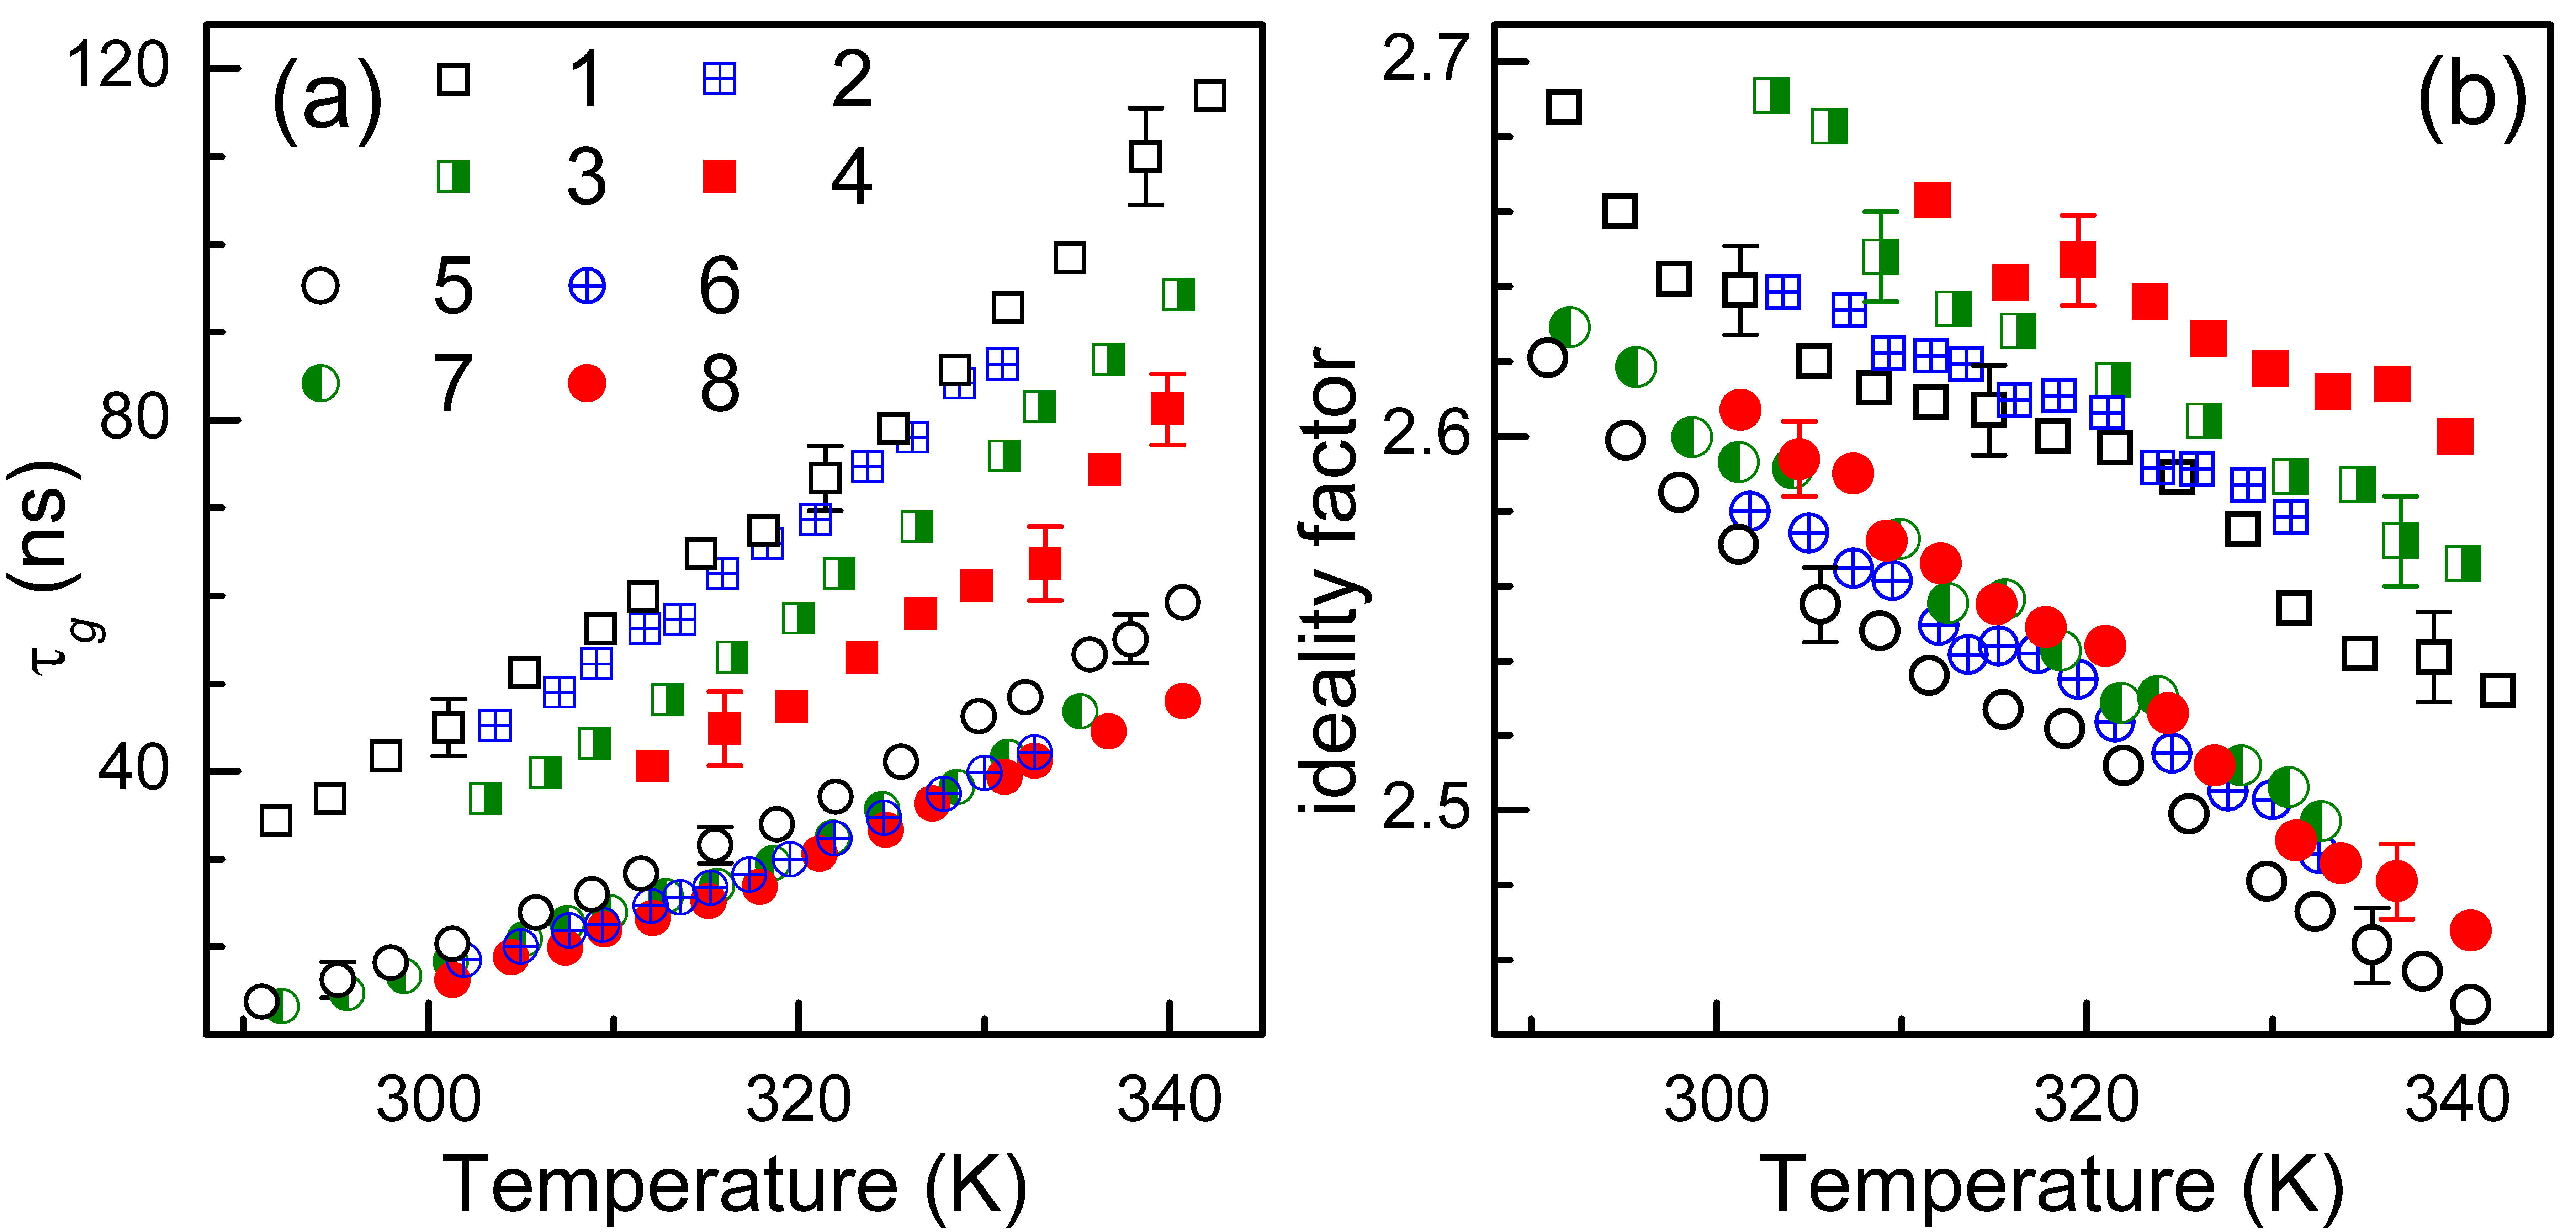
\includegraphics[width=15cm]{olikhFig2ab}%
\end{center}
\caption{\label{figDUS}
%Temperature dependences of SCR carrier lifetime (a), ideality factor (b), base  carrier lifetime (c)
%and shunt resistance (d) with (curves 2--4 and 6--8) and without (1 and 5) USL of
Temperature dependences of SCR carrier lifetime (a) and  ideality factor (b) for the SC--R15 (squares, curves 1--4) and SC--R4 (circles, curves 5--8) with (curves 2--4 and 6--8) and without (1 and 5) USL.
The longitudinal (2, 6) and transverse (3, 4, 7, 8) ultrasound waves were used.
$W_{U\!S}$,W/cm$^2$: 0.18 (2, 6), 0.19 (3), 0.22 (7), 0.40 (4, 8).
}%
\end{figure}


\begin{table}
\caption{\label{tab}USL parameters and acoustically induced changes of SSC parameters.}
\begin{center}
%\begin{ruledtabular}
\begin{tabular}{lcccccc}
\hline
\hline
Sample& \multicolumn{3}{c}{SC--R4}&\multicolumn{3}{c}{SC--R15}\\
Wave type& L & T &  T & L & T &  T\\
$W_{U\!S}$  (W/cm$^2$) &0.18&0.22&0.40&0.18&0.19&0.40\\
$\xi_{U\!S}$  ($10^{-6}$) &1.3&3.1&4.2&1.3&2.8&4.2\\
$u_{U\!S}$  (nm) &0.3&0.7&0.9&0.3&0.6&0.9\\
\hline
$\Delta n$ ($10^{-3}$) &$16\pm10$&$24\pm10$&$28\pm10$&$10\pm10$&$22\pm10$&$43\pm10$\\
%$\Delta n$ ($\pm0.010$) &0.016&0.024&0.028&0.010&0.022&0.043\\
%$\varepsilon_{\tau g}$ ($\pm5$\%)&-12&-14&-17&-5&-18&-30\\
$-\varepsilon_{\tau g}$ (\%)&$12\pm5$&$14\pm5$&$17\pm5$&$5\pm5$&$18\pm5$&$30\pm5$\\
$-\varepsilon_{\tau n}$ (\%)&$11\pm12$&$43\pm12$&$58\pm12$&$13\pm12$&$71\pm12$&$85\pm12$\\
$-\varepsilon_{\tau n}^{Jph}$ (\%)&$2\pm15$&&$39\pm15$&$14\pm15$&&$54\pm15$\\
%$\varepsilon_{\tau n}$ ($\pm12$\%)&-11&-43&-58&-13&-71&-85\\
$K_{U\!S}$ ($10^{6}$ W/cm$^{2}$s)&$0.2\pm0.1$&\multicolumn{2}{c}{$1.0\pm0.2$}&$0.3\pm0.1$&\multicolumn{2}{c}{$6.5\pm0.5$}\\
$-\varepsilon_{Rdis}$ (\%)&0&$23\pm15$&$40\pm15$&--&--&--\\
$-\varepsilon_{Jph}$ (\%)&$0\pm1$&&$9\pm1$&$0\pm1$&&$4\pm1$\\
$-\varepsilon_{Voc}$ (\%)&$3\pm2$&$4\pm2$&$13\pm2$&$2\pm2$&$6\pm2$&$11\pm2$\\
$-\varepsilon_{FF}$ (\%)&$2\pm2$&$2\pm2$&$5\pm2$&$2\pm2$&$3\pm2$&$4\pm2$\\
\hline
\hline
\end{tabular}
%\end{ruledtabular}
\end{center}
\end{table}


Initially, we want to stress, that reversibility of the acoustically driven effects testifies that ultrasound doesn't make change in defect concentration as well as doesn't cause defect diffusion.
Before the causes of ultrasound influence would be discussed, the recombination mechanism must be identified.
Firstly the large ideality factor and small carrier lifetime (about $10^{-8}$~s at room temperature) must be accentuated.
An ideality factor larger than 2 cannot be explained by classical  SRH-theory.
Several attempts to explain large $n$ have been made with various models.
For example, according to van der Heide \emph{et al.}\cite{Heide}, a nonuniform contact resistance of the front side metallisation leads to a high $n$ value.
However, this theory predicts the dependence of ideality factor on light intensity, whereas change of $n$ value with $W_{ph}$ variation is not observed in our case.
Beier and Voss \cite{Beier} explained the large $n$ by  saturation effects within the SRH-model for several donor-like levels.
However, this theory is unable to explain the magnitude of the recombination current $I_{0n}$, which is orders of magnitude larger than expected for silicon.
The high ideality factor was attributed to deep-level-assisted tunneling \cite{Shah,Kaminski_n} too.
But according to this model, the ideality factor is  fairly  constant  versus temperature, whereas such dependencies are observed experimentally --- see \Fref{figDUS}(b).

At the same time, the experimentally observed large $n$ and small $\tau_{g}$ can be explained by the model of coupled defect level recombination \cite{CDLR:JAP1995,CDLR:JAP}.
This model provides a rapid  direct  charge  transfer  between  defect levels.
Initially \cite{CDLR:JAP1995}, it was suggested, that at least one shallow level participated.
Subsequently the model of the donor--acceptor--pair (DAP) recombination (via deep levels) was proposed \cite{CDLR:JAP}.

According to the DAP recombination model both $n$ and $\tau_{g}$ depend on the hole and electron capture cross sections ($\sigma_p$ and $\sigma_n$) as well as on coupling parameter $r_{DA}$.
By-turn, $\sigma_{n,p}$ and $r_{DA}$ depend on the distance between donor and acceptor $r$ and in the simplified case can be expressed as \cite{CDLR:JAP}:
\begin{eqnarray}
\label{eqSigma}
\sigma_{n,p} (r)= \sigma_{n,p}^0\left(\frac{r}{C_r}\right)^2\,,\\
\label{eqRda}
r_{DA} (r)= c_{DA}^0N_DN_A\left[1+\frac{r}{a_0}+\frac{1}{3}\left(\frac{r}{a_0}\right)^2\right]\exp\left(-\frac{r}{a_0}\right)\,,
\end{eqnarray}
where
$\sigma_{n}^0$ and $\sigma_{p}^0$ are capture cross sections of the isolated donor and acceptor,
$N_D$ and $N_A$ are the donor and acceptor concentration,
$a_0$ is the defect Bohr radius,
$C_r$ and $c_{DA}^0$ are some constant.
In particular \cite{CDLR:JAP1995}, if no carrier  exchange  between  the  donor level  and  the valence  band as well as between the  acceptor level  and  the conduction band are assumed then the total recombination rate will be
\begin{equation}
\label{eqR}
R=R_{12}-\sqrt{R_{12}^{\,2}-\frac{np-n_i^2}{\tau_{D,n}\tau_{A,p}(1-\epsilon)}}
\end{equation}
with
\begin{equation}
\label{eqR12}
R_{12}=\frac{(n+n_D)(p+p_A)}{2r_{DA}\tau_{D,n}\tau_{A,p}(1-\epsilon)}+\frac{\tau_{D,n}(p+p_D)+\tau_{A,p}(n+n_A)}{2\tau_{D,n}\tau_{A,p}(1-\epsilon)}\,.
\end{equation}
$\tau_{D,n}\sim 1/\sigma_{n}^{0,D}$ and $\tau_{A,p}\sim 1/\sigma_{p}^{0,A}$ are the electron and hole  lifetimes  for  the non-coupled donor and acceptor respectively,
$n_D$, $p_D$, $n_A$, $p_A$ and $\epsilon$ depend on the energy positions and degeneracy  factors  of  the defect levels \cite{CDLR:JAP1995}.
It is known, that $\tau_{g}\sim R^{-1}$.
Unfortunately, the functional relation between ideality factor and DAP recombination parameters is not suggested,
but $n$ is shown \cite{CDLR:JAP1995,CDLR:SSP} to increase with the $r_{DA}$ and lifetime decrement.

DAP model permits to explain the observed temperature dependencies of both $n$ and $\tau_{g}$ -- see \Fref{figDUS}(a) and \Fref{figDUS}(b).
Actually, the capture cross section of the attractive centers is known \cite{Bube,Sachenko} to depend on temperature as $T^{-1}$ up to $T^{-3}$.
Therefore $\sigma_{n}^{0,D}$ and $\sigma_{p}^{0,A}$ reduce due to the temperature increase and cause the observed changes of the ideality factor and  carrier lifetime.
In addition, the difference in initial $\tau_{g}$ and $n$ values for SC--R15 and SC--R4 (\Fref{figDUS},(a),(b) curves 1 and 5) can deal with large distance between coupled defects.


On our opinion, the reversible ultrasound influence deals with the alteration of the distance between donor and acceptor.
Really, according to \cite{MirzadeJAP2011,PeleshchakUJF2016}, the force acting on the point defect during USL can be expressed as
\begin{equation}
\label{eqFd}
F_d=K\,\Delta\Omega_d\frac{\partial \xi(x,t)}{\partial x}\,,
\end{equation}
where $K$ is the bulk elasticity modulus,
$\Delta\Omega_d$ is volume elastic strain caused by the relaxation of the defect volume (e.g. $\Delta\Omega_d<0$ and $\Delta\Omega_d>0$ for  vacancies and interstitial atoms, respectively),
$\xi$ is the crystal lattice deformation,
and acoustic wave propagates along $x$ direction.
$\partial \xi(x,t)/\partial x$ linearly depends on the deformation amplitude $\xi_{U\!S}=\sqrt{2W_{U\!S}/\rho_{Si}\,\vartheta_{U\!S}^3}$
(where $\rho_{Si}=2.33$~g/m$^3$ is the silicon density,
$\vartheta_{U\!S}$ is the ultrasound velocity, equals to $9850$~m/s and $5840$~m/s for longitudinal and transverse wave respectively).
Therefore, a point defect vibrates under USL condition and oscillation amplitude and phase are determined by both defect character and acoustic wave intensity and type.

\begin{figure}
\begin{center}
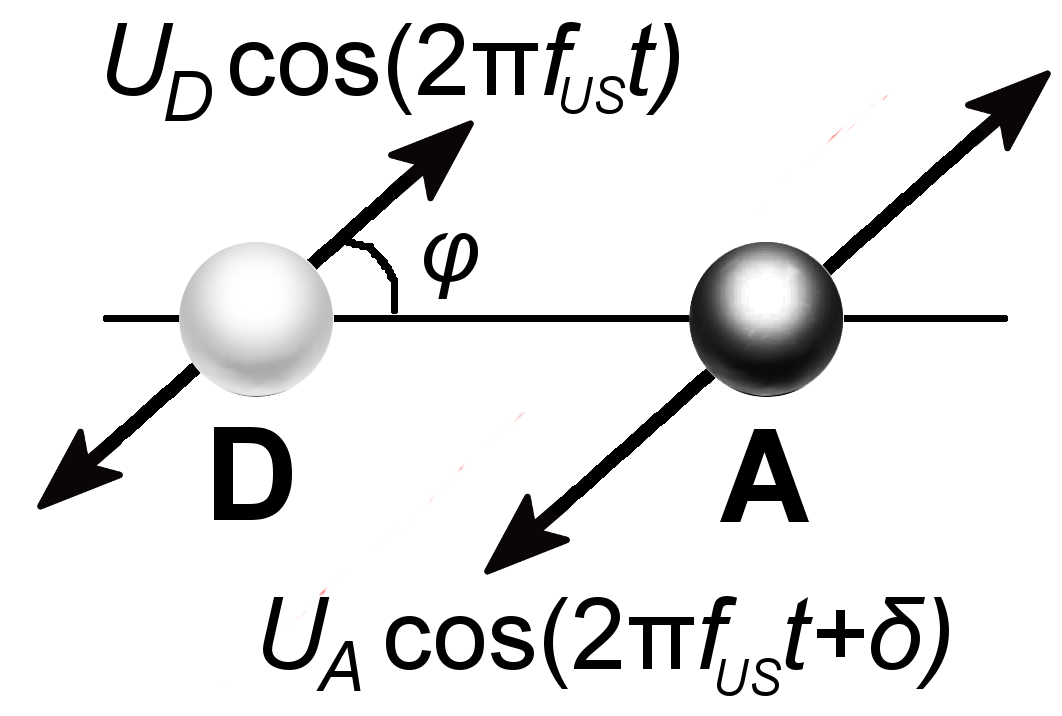
\includegraphics[width=7.5cm]{olikhFig3}%
\end{center}
\caption{\label{figModel}
Behavior of DAP recombination center under USL condition.
}%
\end{figure}

Some qualitative conclusion can be drawn from the simplest model, which is shown on \Fref{figModel}.
Initially two point defect, donor (D) and acceptor (A) are situated at distance $r_0$.
During USL defects would vibrate with amplitudes $u_D$ and $u_A$.
%Two point defect, donor (D) and acceptor (A) vibrates under ultrasound action with amplitudes $u_D$ and $u_A$.
The amplitudes depend on $\xi_{U\!S}$, defect elastic strain ($\Delta\Omega_D$ and $\Delta\Omega_A$), defect coupling  and can be different.
$\delta$ is the phase shift between donor and acceptor vibration.
If no ultrasound energy absorption by defect is assumed,
then $\delta$ will equal to $0^\circ$ and $180^\circ$ in the case of $\Delta\Omega_D\cdot\Delta\Omega_A>0$ and  $\Delta\Omega_D\cdot\Delta\Omega_A<0$ respectively.
$\varphi$ is the angle between the defect pair axis and the forced displacement direction.

\begin{figure}
\begin{center}
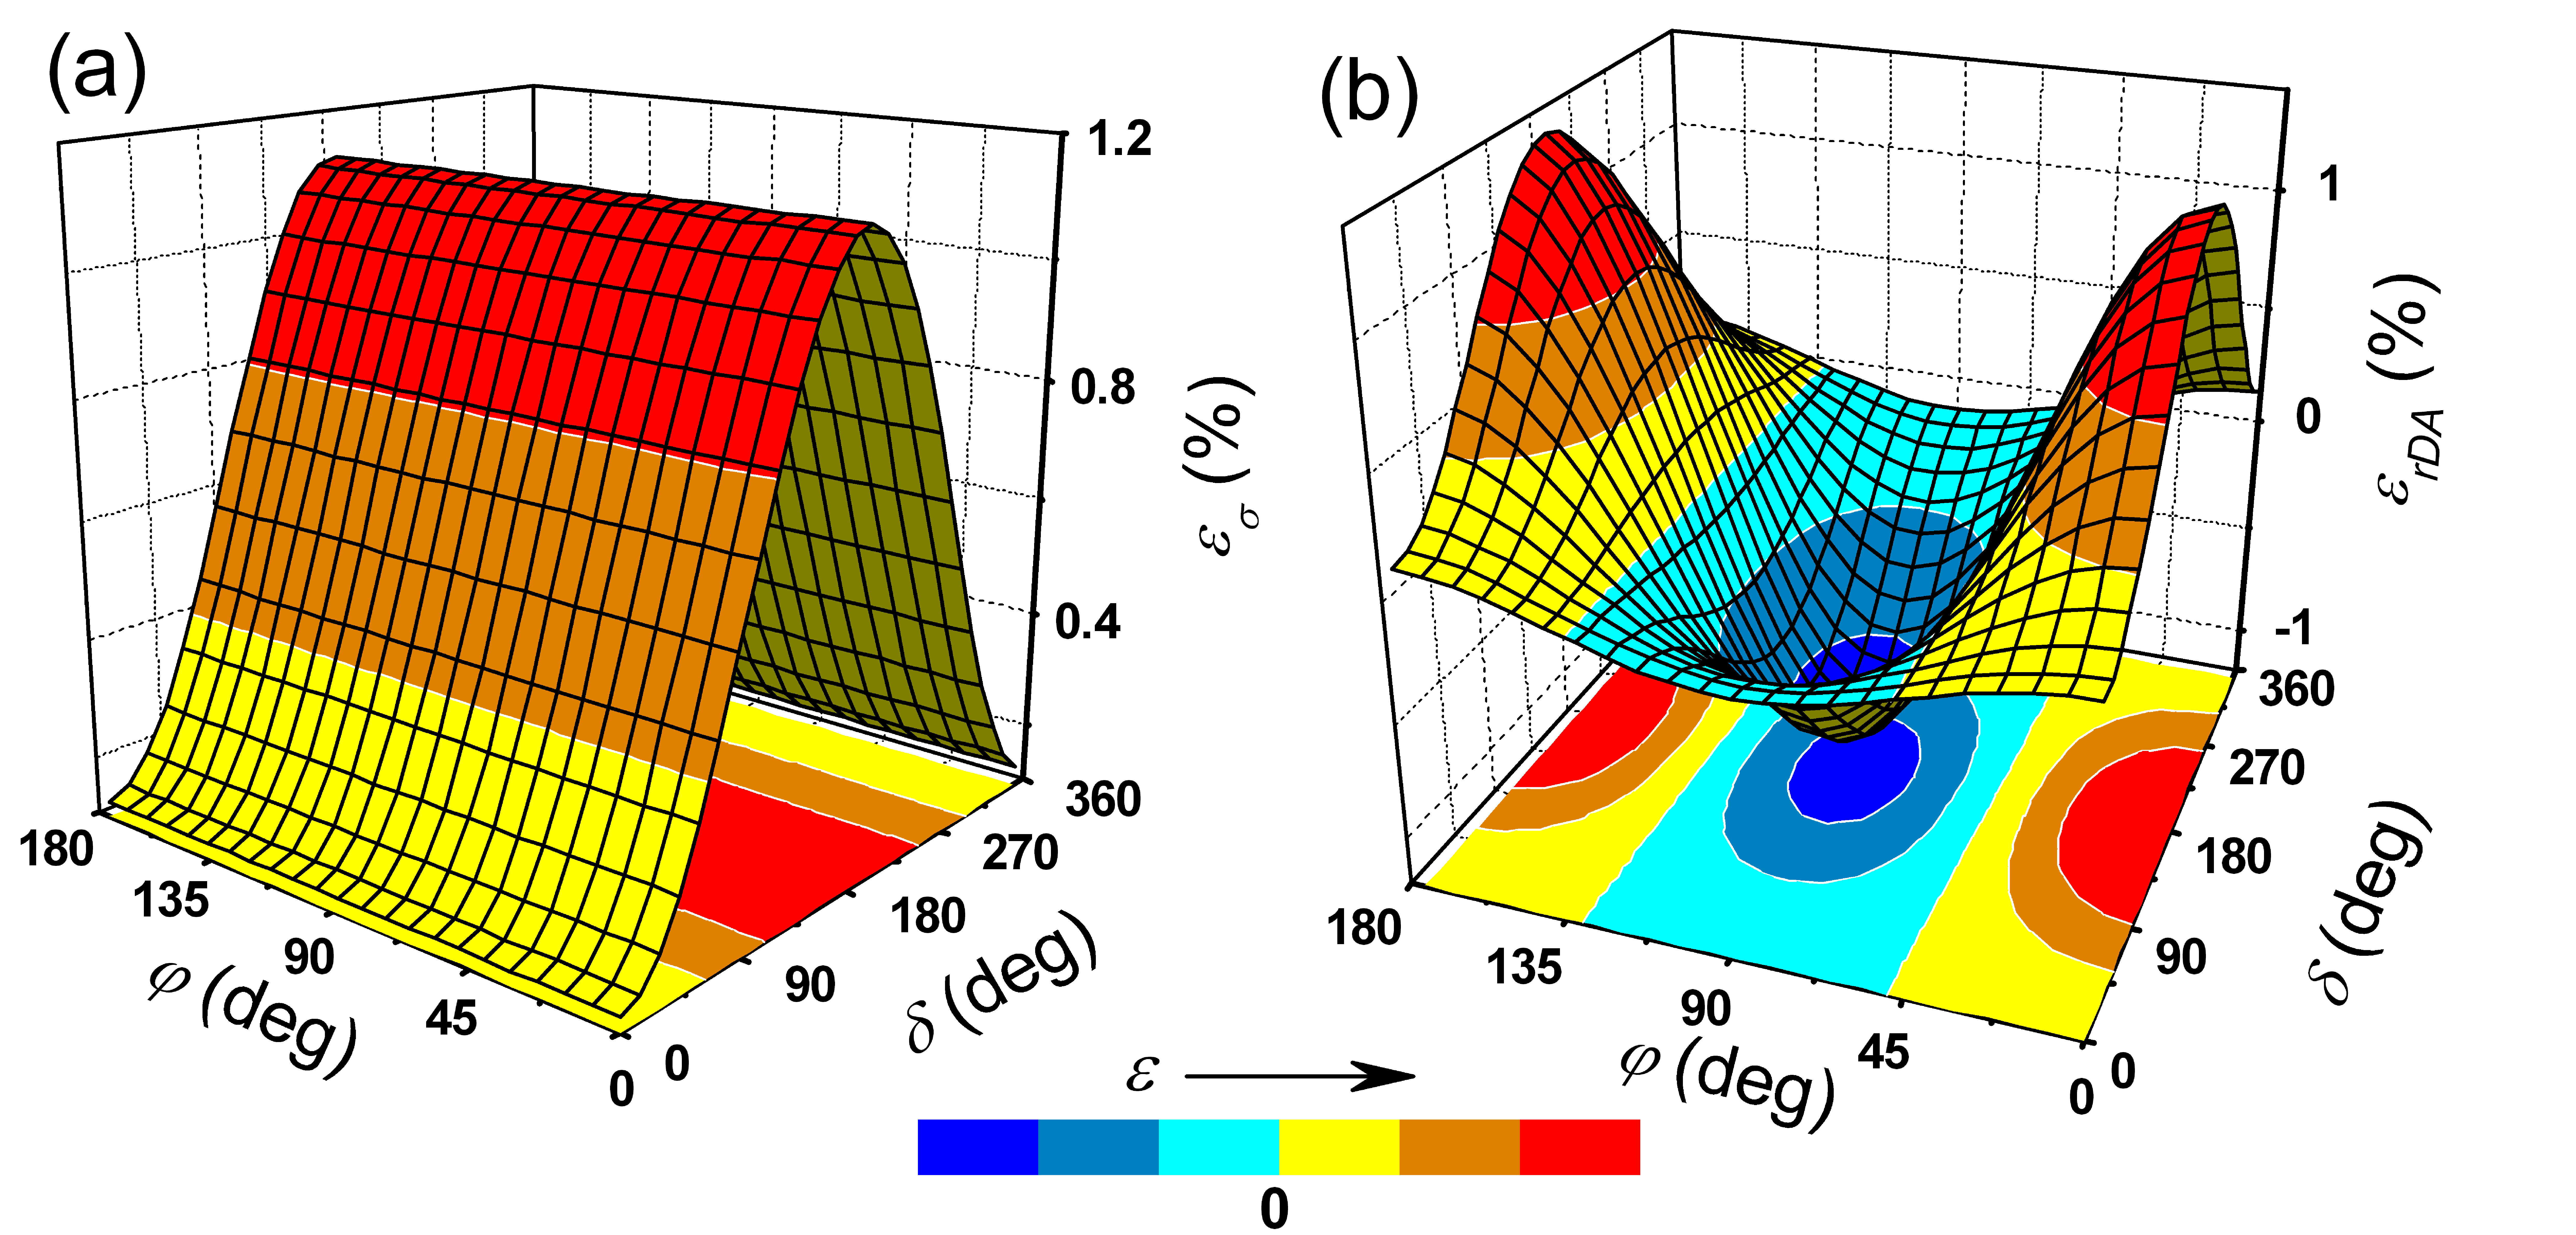
\includegraphics[width=14cm]{olikhFig4ab}%
\end{center}
\caption{\label{figR2L}
Simulated dependencies of AI changes of capture cross section (a) and coupling parameter (b) on the vibration phase shift  and on the angle between the pair axis and the displacement direction.
The parameters are set to $a_0=3.23$~nm, $r_0=10$~nm, $u_A=1$~nm, $u_D=0.5$~nm.
}%
\end{figure}

\begin{figure}
\begin{center}

\includegraphics[width=14cm]{olikhFig5ab}%
\end{center}
\caption{\label{figLnew}
Simulated dependencies of AI changes of coupling parameter on the vibration amplitudes  and on initial distance between donor and acceptor.
The parameters are set to $\varphi=0^\circ$, $\delta=0^\circ$ (a) and $\varphi=90^\circ$, $\delta=180^\circ$ (b).
}%
\end{figure}

Generally,  the distance $r$ between donor and acceptor would not equal to $r_0$ during vibration.
\Fref{figR2L} and \Fref{figLnew} show relative changes of capture cross section $\varepsilon_{\sigma}=[\sigma(r)-\sigma(r_0)]/\sigma(r_0)$ and coupling parameter $\varepsilon_{r_{DA}}=[r_{DA}(r)-r_{DA}(r_0)]/r_{DA}(r_0)$.
$\varepsilon_{\sigma}$ and $\varepsilon_{r_{AD}}$ are averaged over the ultrasound wave period.
Under simulation
(i)~it was assumed, that relaxation time in the recombination sub-system was considerably less than $f_{U\!S}^{-1}$;
(ii)~Eqs. (\ref{eqSigma}) and (\ref{eqRda}) were used;
(iii)~the value $a_0=3.23$~nm from the \cite{CDLR:JAP} was utilized;
(iv)~the chosen $u_D$ and $u_A$ values were commensurate with the atom displacement $u_{U\!S}$ in acoustic wave (see Table~\ref{tab}).
Simulations show that the extent of ultrasound influence on both $r_{DA}$ and $\sigma$ increases with $r_0$ decrease.
In simple cases $\delta=0^\circ$ or $\delta=180^\circ$,
the amplitude dependencies of $\varepsilon_{\sigma}$ and $\varepsilon_{r_{DA}}$ are determined by $|u_D-u_A|$ and $(u_D+u_A)$ respectively.
In particular
\begin{equation}
\label{eqEpsSig}
\varepsilon_{\sigma}=\frac{(u_D\pm u_A)^2}{2r_0^2}\,.
\end{equation}


\Fref{figR2L}(a) and Eq.~(\ref{eqEpsSig}) show that the capture cross section increases under USL condition.
AI alteration of coupling parameter is more complicated and sign of $\varepsilon_{r_{DA}}$ depends on $\varphi$ and $r_0$ - see \Fref{figR2L}(b) and \Fref{figLnew}.
But in the case of low $r_0/a_0$ value, DAP recombination is expected \cite{CDLR:JAP1995,CDLR:JAP} to be effective and the AI $r_{DA}$ reduction is forecasted by \Fref{figLnew} even through  $\varphi=0^\circ$.

According to the DAP recombination theory,  $\sigma$ increase and $r_{DA}$ decrease must cause a lifetime reduction and an ideality factor rise.
Just so effects are observed under USL condition.
Under equal $W_{{U\!S}}$ value conditions T--USL is more effective due to the larger $\varepsilon_{U\!S}$ value (see Table~\ref{tab}).
As mentioned above, the $r_0$ is probably smaller in SC--R15 than in SC--R4.
On our opinion, it is a reason of the more remarkable AI effect in SC--R15.

\subsection{Ultrasound influence on recombination in the SSC base}

\begin{figure}
\begin{center}
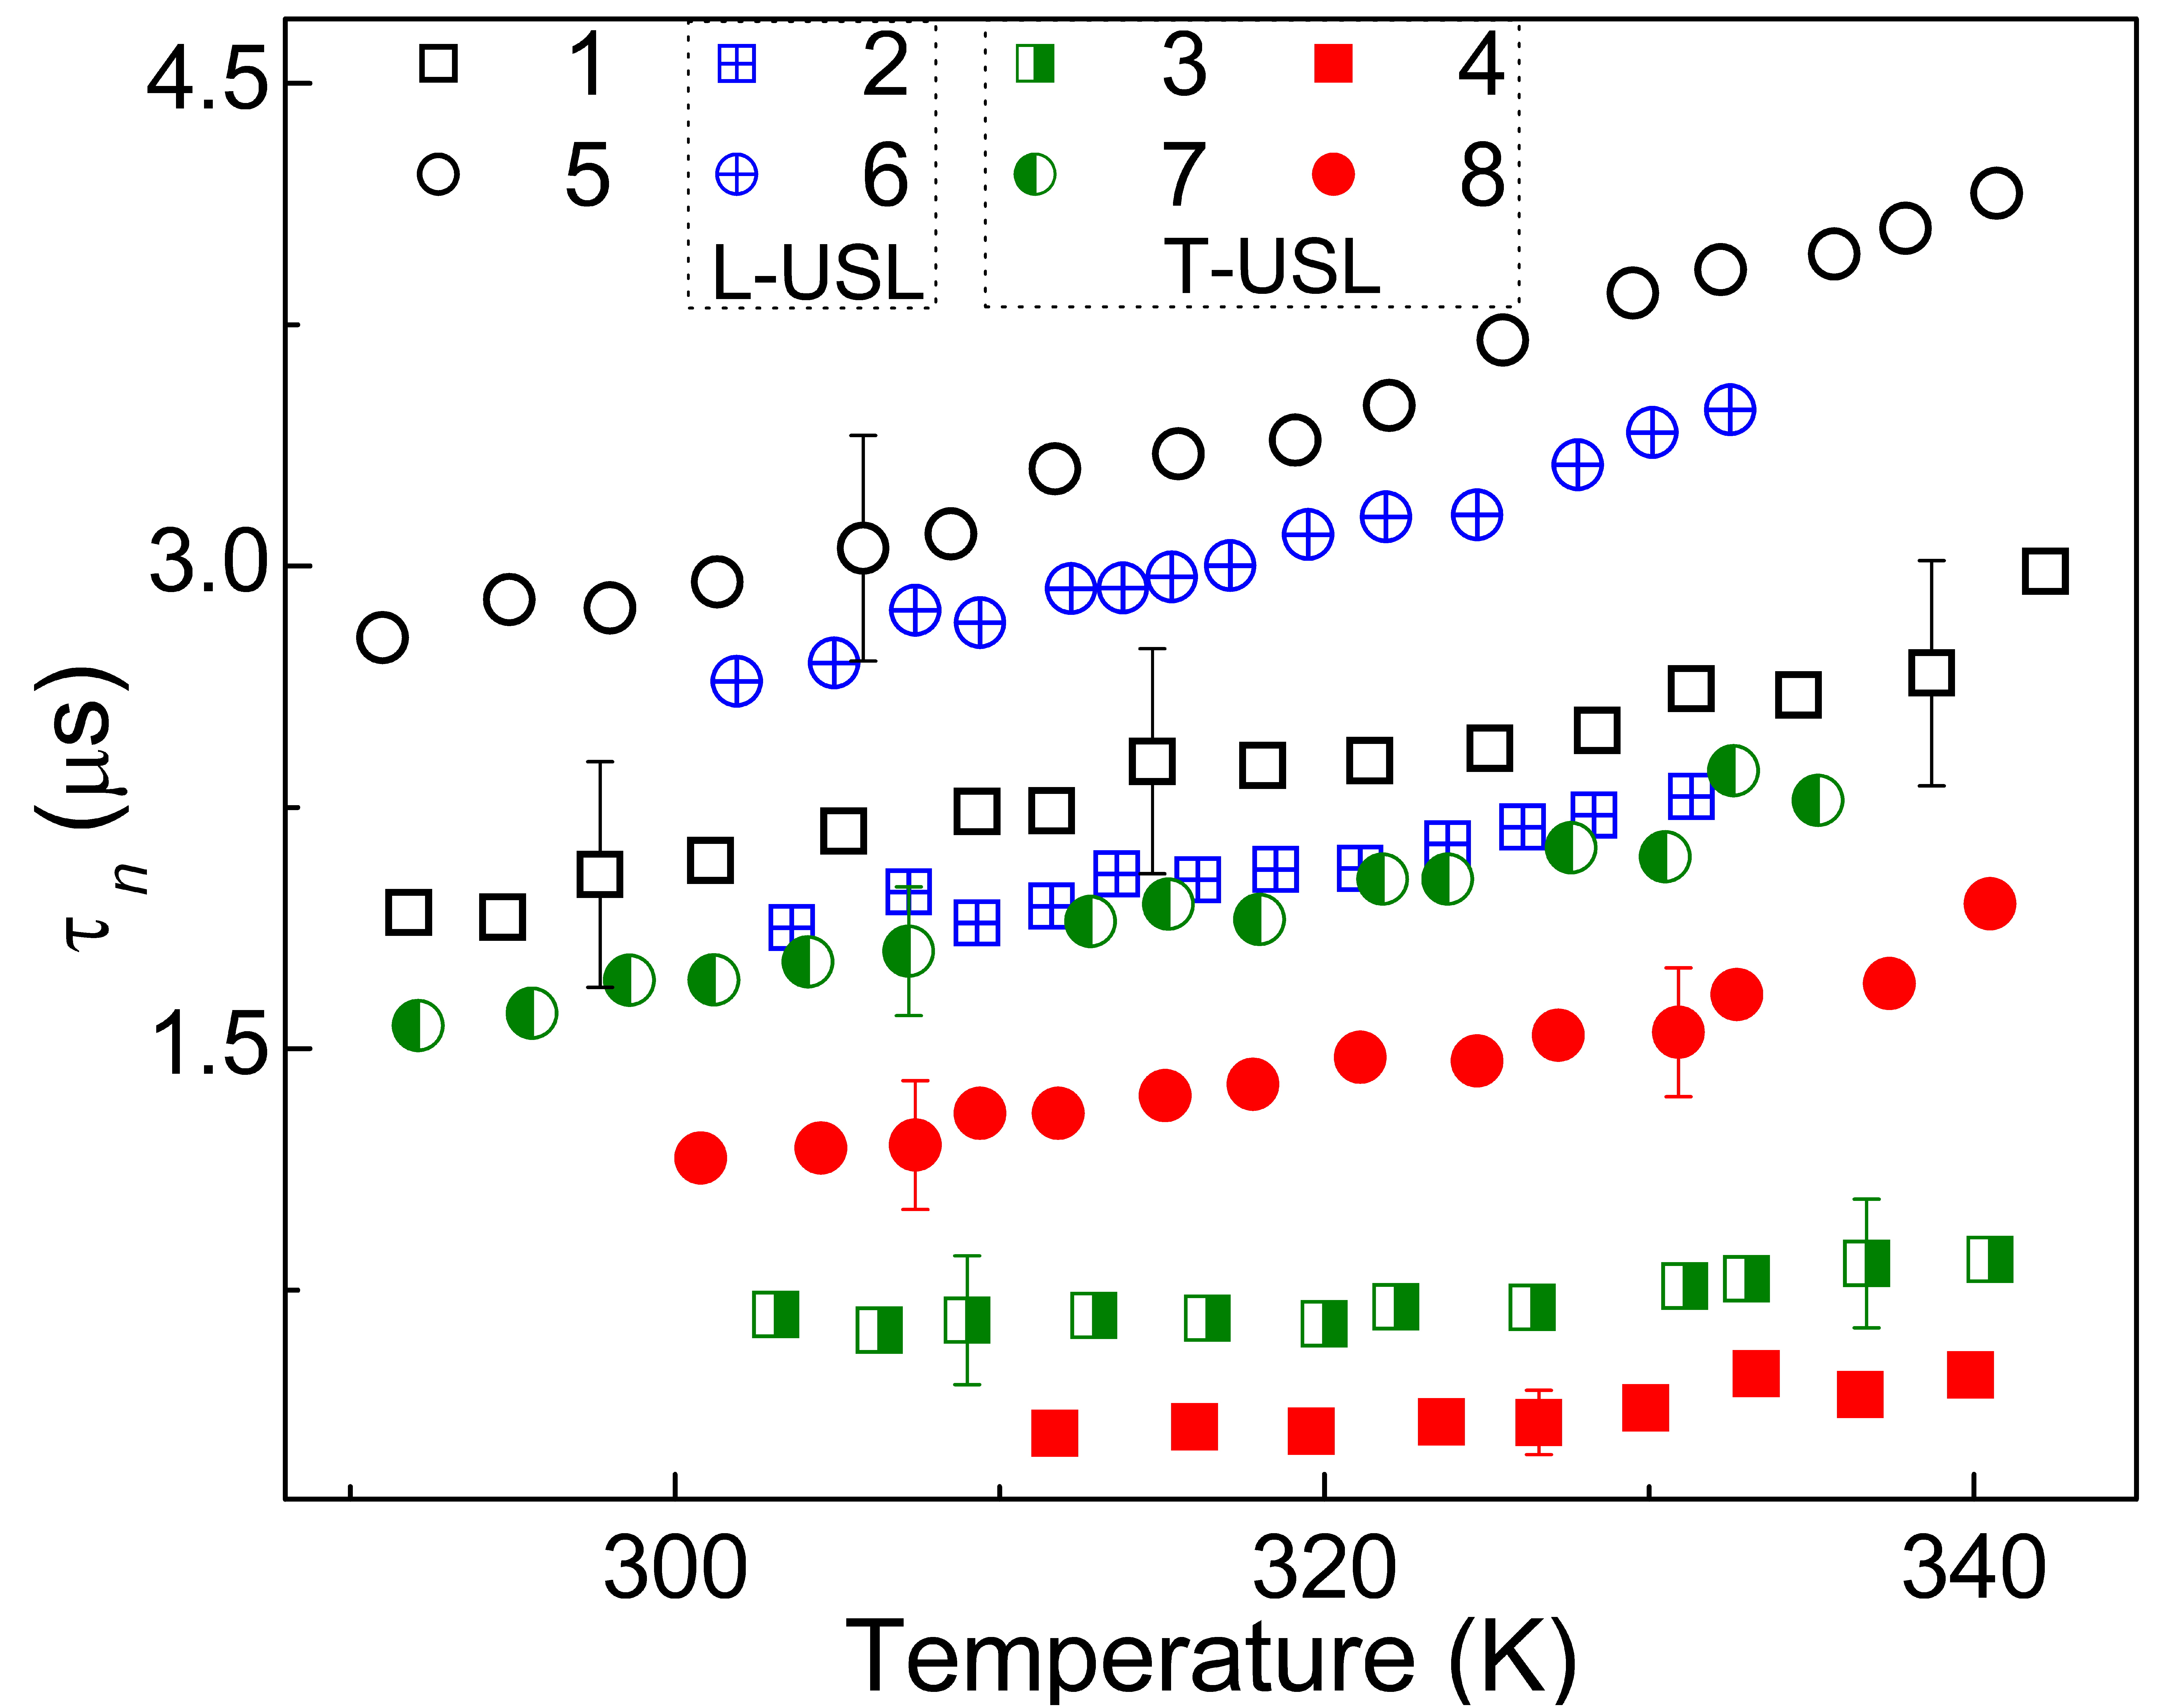
\includegraphics[width=7.5cm]{olikhFig6}%
\end{center}
\caption{\label{figDUS_Tau}
Temperature dependencies of base  carrier lifetime for
the SC--R15 (squares, 1--4) and SC--R4 (circles, 5--8) with (2--4 and 6--8) and without (1 and 5) USL.
%The longitudinal (2, 6) and transverse (3, 4, 7, 8) ultrasound waves were used.
$W_{U\!S}$,W/cm$^2$: 0.18 (2, 6), 0.19 (3), 0.22 (7), 0.40 (4, 8).
}%
\end{figure}

Temperature dependencies of the minority carrier lifetime in the p--region of SSC are shown in \Fref{figDUS_Tau}.
The SRH lifetime due a defect in p--type material at low injection level can be written as
\begin{equation}
\label{eqSRH_tau}
\tau_n=(N_d\sigma_n\nu_{th})^{-1}\,,
\end{equation}
where $N_d$ is the concentration of the defect, $\nu_{th}$ is the thermal velocity.
To our mind, the slight increment of $\tau_n$ with $T$ results from the $\sigma_n$ temperature dependency, which is mentioned above.
As one can see, the USL causes the lifetime $\tau_n$ decrease, that runs down to 20\% of $\tau_n$ initial value.
The relative AI change of an electron lifetime $\varepsilon_{\tau n}$ is presented in Table~\ref{tab}.

\begin{figure}
\begin{center}

\includegraphics[width=7.5cm]{olikhFig7}%
\end{center}
\caption{\label{figMS}
Dependencies of reciprocal lifetime in the SSC base on ultrasound intensity for the SC--R4 (circles, left axis) and SC--R15 (squares, right axis) at 320~K.
Symbol filling is defined by the intensity and type of ultrasound waves and coincides with \Fref{figDUS_Tau} notation.
Lines are linear fitting of T--USL data.
}%
\end{figure}

Ordinary the lifetime reduction under radiation action is described by the Messenger�-Spratt equation \cite{Markvart}:
\begin{equation}
\label{eqMS}
\tau_n^{-1}=\tau_{n0}^{-1}+K\Phi\,,
\end{equation}
where $\tau_{n0}$ is the minority carrier lifetime in the unirradiated cell,
$\Phi$ is the integrated flux,
and $K$ is a lifetime damage constant characteristic for the material and the type of irradiation.
The dependencies of reciprocal lifetime on ultrasound intensity are shown on \Fref{figMS}.
As one can recognize, the linear dependence of $1/\tau_n$ on $W_{{U\!S}}$  is observed.
Therefore the modified Messenger�-Spratt equation can be used to describe the acoustically driven  change of the lifetime:
\begin{equation}
\label{eqMS_Us}
\tau_n^{-1}=\tau_{n0}^{-1}+K_{U\!S}W_{U\!S}\,,
\end{equation}
where $\tau_{n0}$ is the lifetime in the ultrasound-free cell and
$K_{U\!S}$ depends on a wave type and a sample state.
The defined $K_{U\!S}$ values are listed in Table~\ref{tab}.
Taking into account Eq.~(\ref{eqSRH_tau}) and reversibility of ultrasound influence, we assume the observed decrement in lifetime to be evident of AI change of $\sigma_n$.
In this case the following relation can be obtained by using Eqs.~(\ref{eqSRH_tau}) and (\ref{eqMS_Us}):
\begin{equation}
\label{eqTau}
\frac{\varepsilon_{\sigma}}{\tau_{n0}W_{U\!S}}=K_{U\!S}\,.
\end{equation}

The most recombination centers in the silicon are known to be a complex defect, which is composed of non-equivalent components.
For example, the complexes of two point defects with an opposite charge occur quite often.
Following the empirical relation proposed in \cite{CDLR:R2}, we believe, that the capture cross section of such pair depends on distance between complex's component and Eq.~(\ref{eqR}) is true.
Hence the introduced in Sec.~\ref{P1} model of AI increase of $\sigma$ is applicable to account for $\tau_{n}$ decrease.
Really, according to the model $\varepsilon_{\sigma}\sim u_{D,A}^2\sim \xi_{U\!S}^2\sim W_{U\!S}$, i.e. the linear $\tau_n^{-1}$--$W_{U\!S}$ relation is expected and is observed --- see \Fref{figMS}.
The $K_{U\!S}$ increment in the T--USL and SC--R15  cases (Table~\ref{tab}) relates to the larger $\xi_{U\!S}$--$W_{U\!S}$ proportionality coefficient and smaller $\tau_{n0}$ value respectively.
It should be noted that an initial distance between components of recombination center is much smaller than the distance between participants of DAP recombination;
therefore according to Eq.~(\ref{eqEpsSig}), the more effective ultrasound influence is expected.

\subsection{Light and annealing influence on the SSC parameters
\label{P3}}

Any concrete defect title was not referred as an recombination center in the discussion above.
The additional investigations are necessary to define the type of defects, which are involved in both the recombination and the acousto--defect interaction.

It is known that the most harmful recombination centers in boron--doped Czochralski--grown SSC are the  boron--oxygen related defects \cite{MurphyJAP2011,Kim,LID:BothePP,LIDRev}, iron--boron pairs \cite{MurphyJAP2011,FeB:Vahanissi,FeB:Schmidt} (or another Fe--related trap in the $n^+p$--junctions \cite{TeimurazPSS,TeimurazJAP}), and oxide precipitates \cite{MurphySC2014,Oxide_Schon,MurphyJAP2011,MurphyJAP2012,Oxide:Chen}.
The first two defects are sensitive to an intensive illumination at room temperature.
Thus transformation of boron--oxygen defects by an illumination leads to minority--carrier lifetime degradation (down to as 5 times as small \cite{LIDRev}).
Full lifetime recovery is observed after annealing at 200~$^\circ$C for $10$~min in the dark.
The degradation--recovery cycle can be reiterated \cite{Kim}.
On the other hand, at room temperature, the vast majority of iron exists in iron--boron pairs, which can be readily dissociated under intense illumination to release interstitial iron.
This gives a lifetime change which depends on doping concentration and excess carrier concentration \cite{FeB:Schmidt}.
After the dissociation procedure, the concentration of Fe$_i$ decreases according to \cite{MurphyJAP2011}
\begin{equation}
\label{eqFeB}
N_{Fe}(t)=(N_{Fe,0}-N_{Fe,eq})\exp\left[-1.3\cdot10^{-3}p_p^{\,2/3}\exp\left(-\frac{0.68}{kT}\right)t\right]+N_{Fe,eq}\,,
\end{equation}
where
$N_{Fe,0}$ and $N_{Fe,eq}$ are the concentration after dissociation immediately and equilibrium
concentration which remains a long time after dissociation respectively.



To inspect an availability of boron--oxygen defects and iron--boron pairs the following experimental procedure has been used.
The samples were light soaked under halogen lamp (2 Suns) illumination at approximately 305~K.
The illumination time varied from 1~h to 8~h.
After illumination samples are stored in the dark at room temperature.
To determine the kinetics of SSC parameters the dark $I$--$V$ characteristics have been measured with interval 10--15~min at room temperature over a period 5~h after illumination stopping.
To determine the permanent LID of SSC parameters the dark $I$--$V$ characteristics have been measured in 48~h after illumination.
After accumulated time under illumination had reached 10--15~h the samples were annealed at 200~$^\circ$C for $10$~min in the dark and SSC parameters were determined at room temperature.
After that, the illumination--annealing cycle was repeated.

The results of residual influence of both illumination and annealing on an equilibrium value of SSC parameters are presented on \Fref{figLight}.
In contrast to other Figures, this contains sample SC--R3 data.
The SC--R3 distinctive features are a low $R_{sh}$ value and a performance of annealing before illumination.
Though the obtained results for SC--R3 are similar to other samples.
One can see that the illumination does not affect a SCR carrier lifetime as well as a base carrier lifetime neither before annealing, nor after.
Illumination induced decrease of ideality factor is commensurable with an accuracy of $n$ determination.
Change of shunt resistance under illumination is most considerable but it reaches $-20$~\% only and does not recur after an  annealing -- see \Fref{figLight}(d), curve for the sample SC--R4.
Annealing had more efficient influence on SSC parameters and results in  an increment of $\tau_g$ and $R_{sh}$ as well as in a decrement of $\tau_n$ and $n$.
Such behavior of SSC parameters under illumination and annealing action is evident of absence of boron--oxygen defects influence.
The reason of light induced and annealing induced changes  will not be further discussed since this is beyond scope of our study.


\begin{figure}
\begin{center}
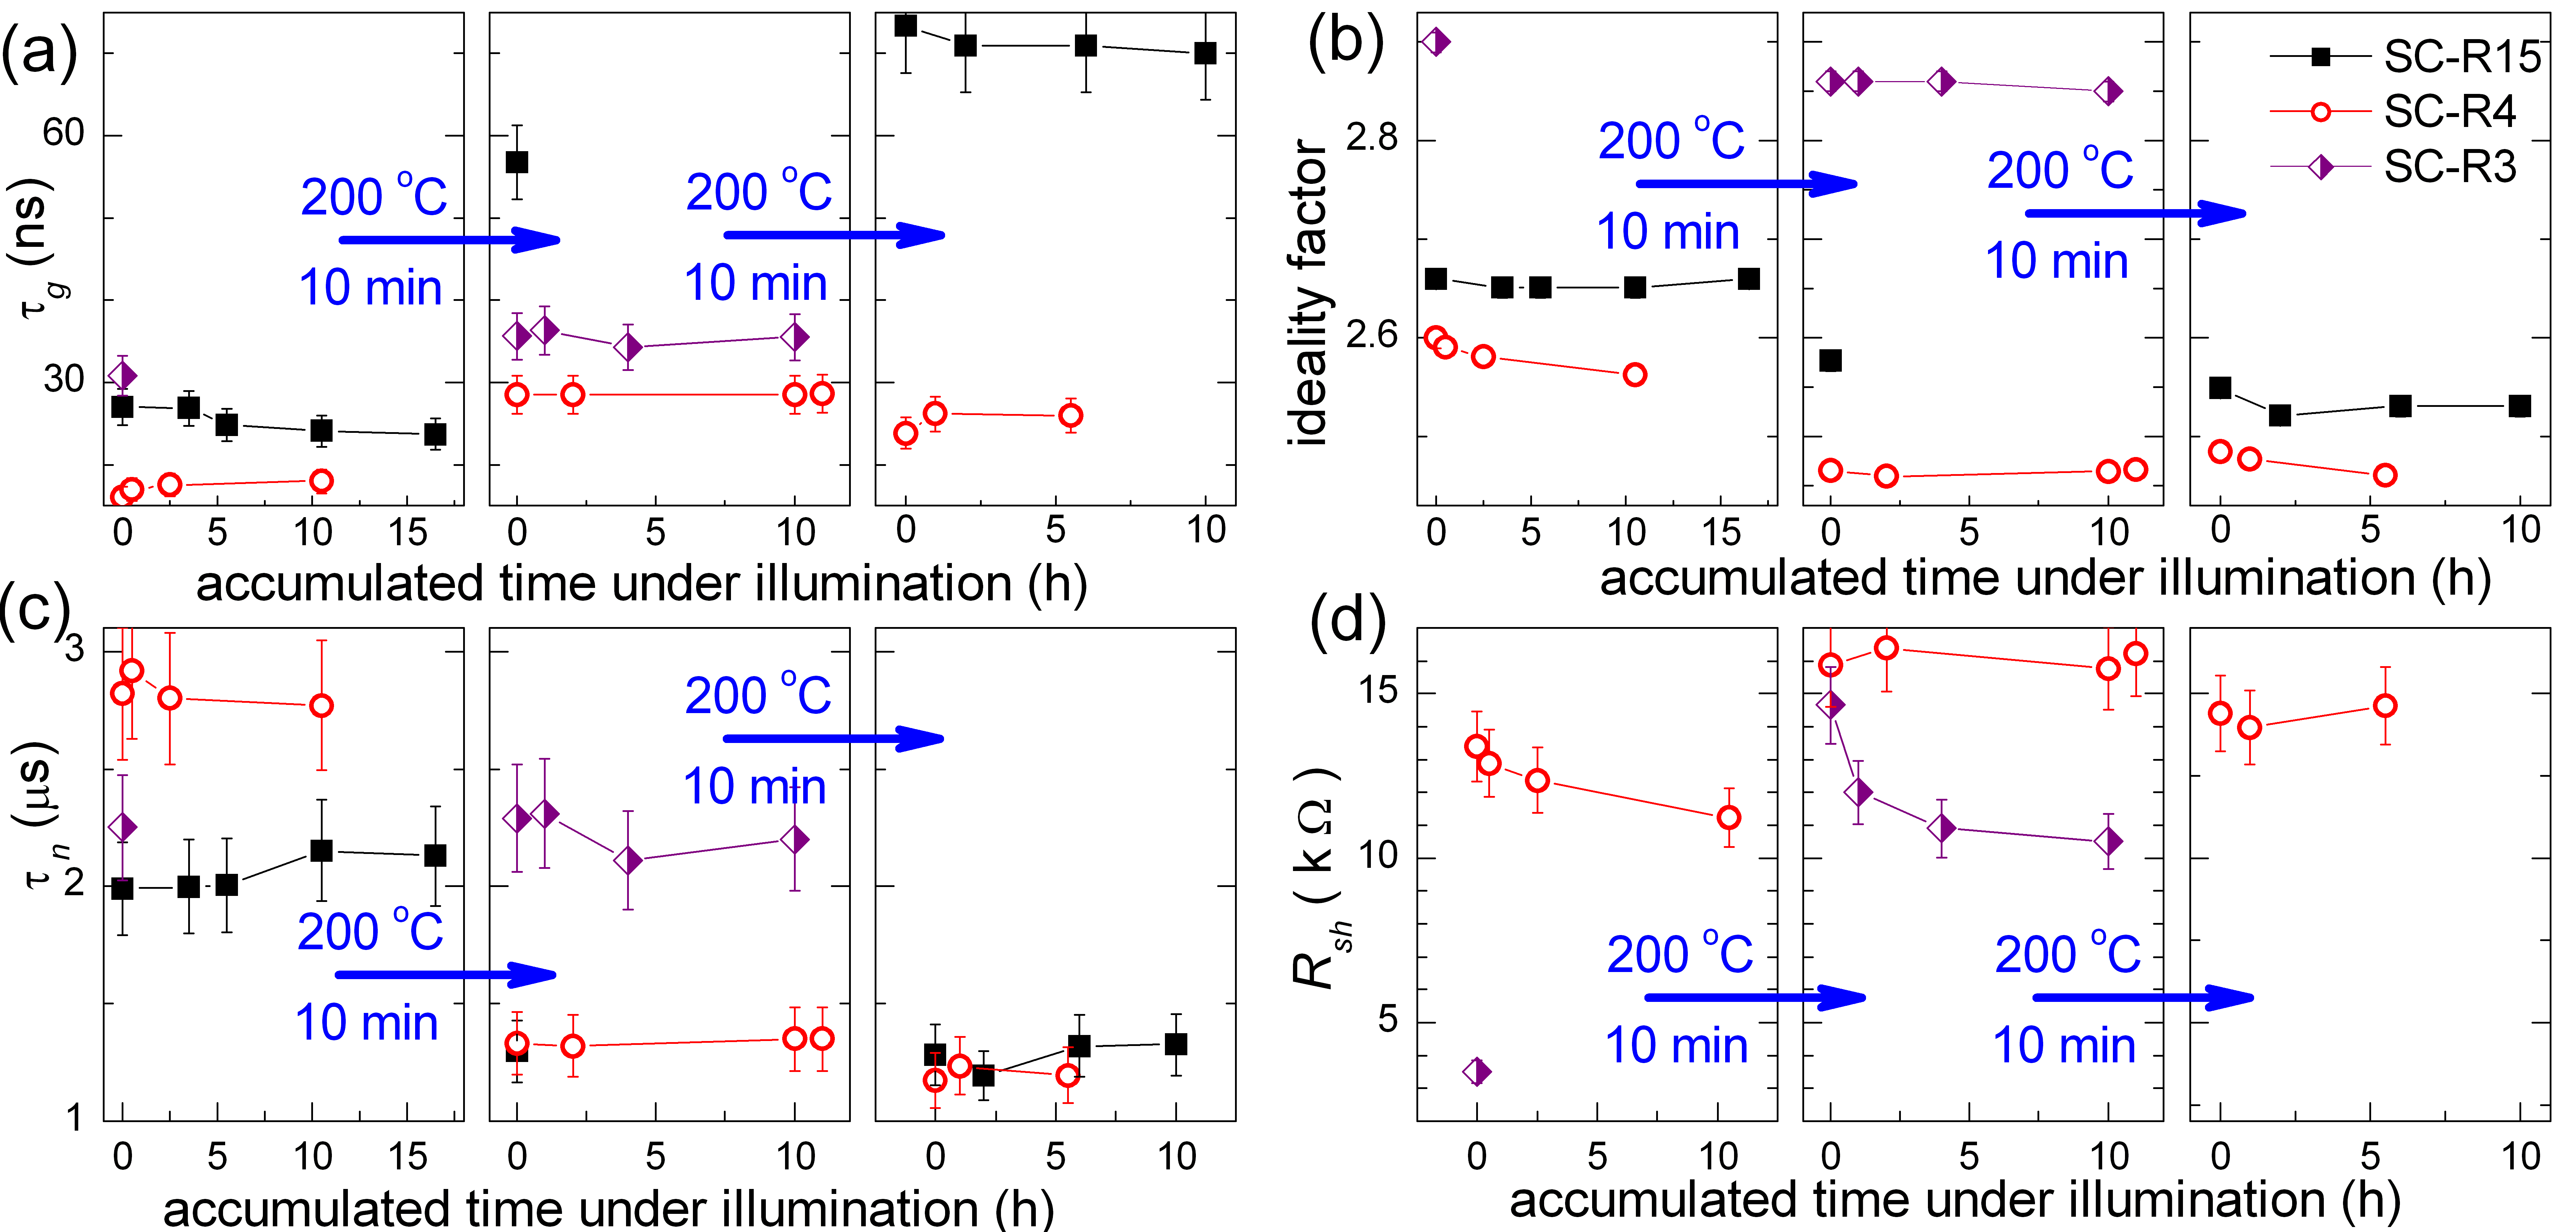
\includegraphics[width=15cm]{olikhFig8abcd}%
\end{center}
\caption{\label{figLight}
Dependencies of SCR carrier lifetime (a), ideality factor (b), base  carrier lifetime (c), and shunt resistance (d) on accumulated illumination time and annealing.
Data were obtained from $I$--$V$ curves which had measured in 48~h after illumination or annealing at $T=295$~K.
Lines only serve as guide to the eye.
}%
\end{figure}

The typical dependencies of SSC parameters versus time since illumination stoping are shown on \Fref{figAfter}.
As one can see, $\tau_n$ and $R_{sh}$ do not vary practically.
Hence these parameters can not be influenced by iron--boron pairs.
At the same time  $\tau_g$ and $n$ are changing after illumination.
We supposed that the expressions, that have described the both $\tau_g$ and $n$ evolution, were similar to    Eq.~(\ref{eqFeB}) and used the characteristic time $\left[1.3\cdot10^{-3}(1.4\times10^{15})^{\,2/3}\exp\left(-\frac{0.68}{295k}\right)\right]^{-1}=2.53\cdot10^4$~s to plot fitting line on \Fref{figAfter}(a) and (b).
The fitting is in good agreement with experimental data.
Therefore pairs Fe$_i$B$_s$ can affect a SCR recombination and the acceptor level $E_C-0.23$~eV can be involved in a DAP recombination process.
Incidentally, pair Fe$_i$B$_s$ is a good candidate for acousto-active defect:
the B is substitutional atom whose volume is smaller than the volume of the matrix atom and $\Delta\Omega_d (\mbox{B}_s)<0$ whereas the interstitial Fe leads to $\Delta\Omega_d (\mbox{Fe}_i)>0$.
On the other hand, the  $\tau_g$ change after illumination is about 10~\% (see \Fref{figAfter}(a)), whereas a capture cross sections change, which is expected due to pair dissociation, equals to 1.7~times for electrons and 0.04~times for holes \cite{FeB:Schmidt}.
Hence, on our opinion, the pair Fe$_i$B$_s$ is not main reason of a SCR recombination in the investigated samples.


\begin{figure}
\begin{center}

\includegraphics[width=7.5cm]{olikhFig9abcd}%
\end{center}
\caption{\label{figAfter}
SCR carrier lifetime (a), ideality factor (b), base  carrier lifetime (c), and shunt resistance (d) as a function of time since illumination stoping.
Sample SC--R4.
$T=295$~K.
Lines are plotted by using Eq.~(\ref{eqFeB}) and characteristic time $2.53\cdot10^4$~s.
}%
\end{figure}


According to Murphy \emph{et al}.\cite{MurphySC2014,MurphyJAP2012},
the recombination at oxide precipitates cannot be explained by a single two--level defect alone and at least two independent defects are exist.
These defects have single energy levels at $E_V+0.22$~eV and $E_C-0.08$~eV and have $\sigma_n/\sigma_p=157$ and $\sigma_p/\sigma_n=1200$ respectively \cite{MurphyJAP2012}.
So, these defects are suitable for the DAP recombination process.
Dislocations and stacking faults surround  the oxide precipitates and lead to capture coefficient change as well as to increase the concentrations of two defects, without introducing additional states into the bandgap \cite{MurphySC2014,MurphyJAP2011,MurphyJAP2012} and can provide their acousto--activity.
The oxide precipitates are nonuniformly distributed across a Cz--Si wafer \cite{Oxide_Schon} or a solar cell \cite{Oxide:Chen} and it is the probable reason for a SSC parameters variation from one investigated sample to another.
On the basis of mentioned above, we conclude that the defects, involved in both recombination and acousto--defect interaction are oxide precipitates mainly.


\subsection{Ultrasound influence on shunt resistance}

\begin{figure}
\begin{center}
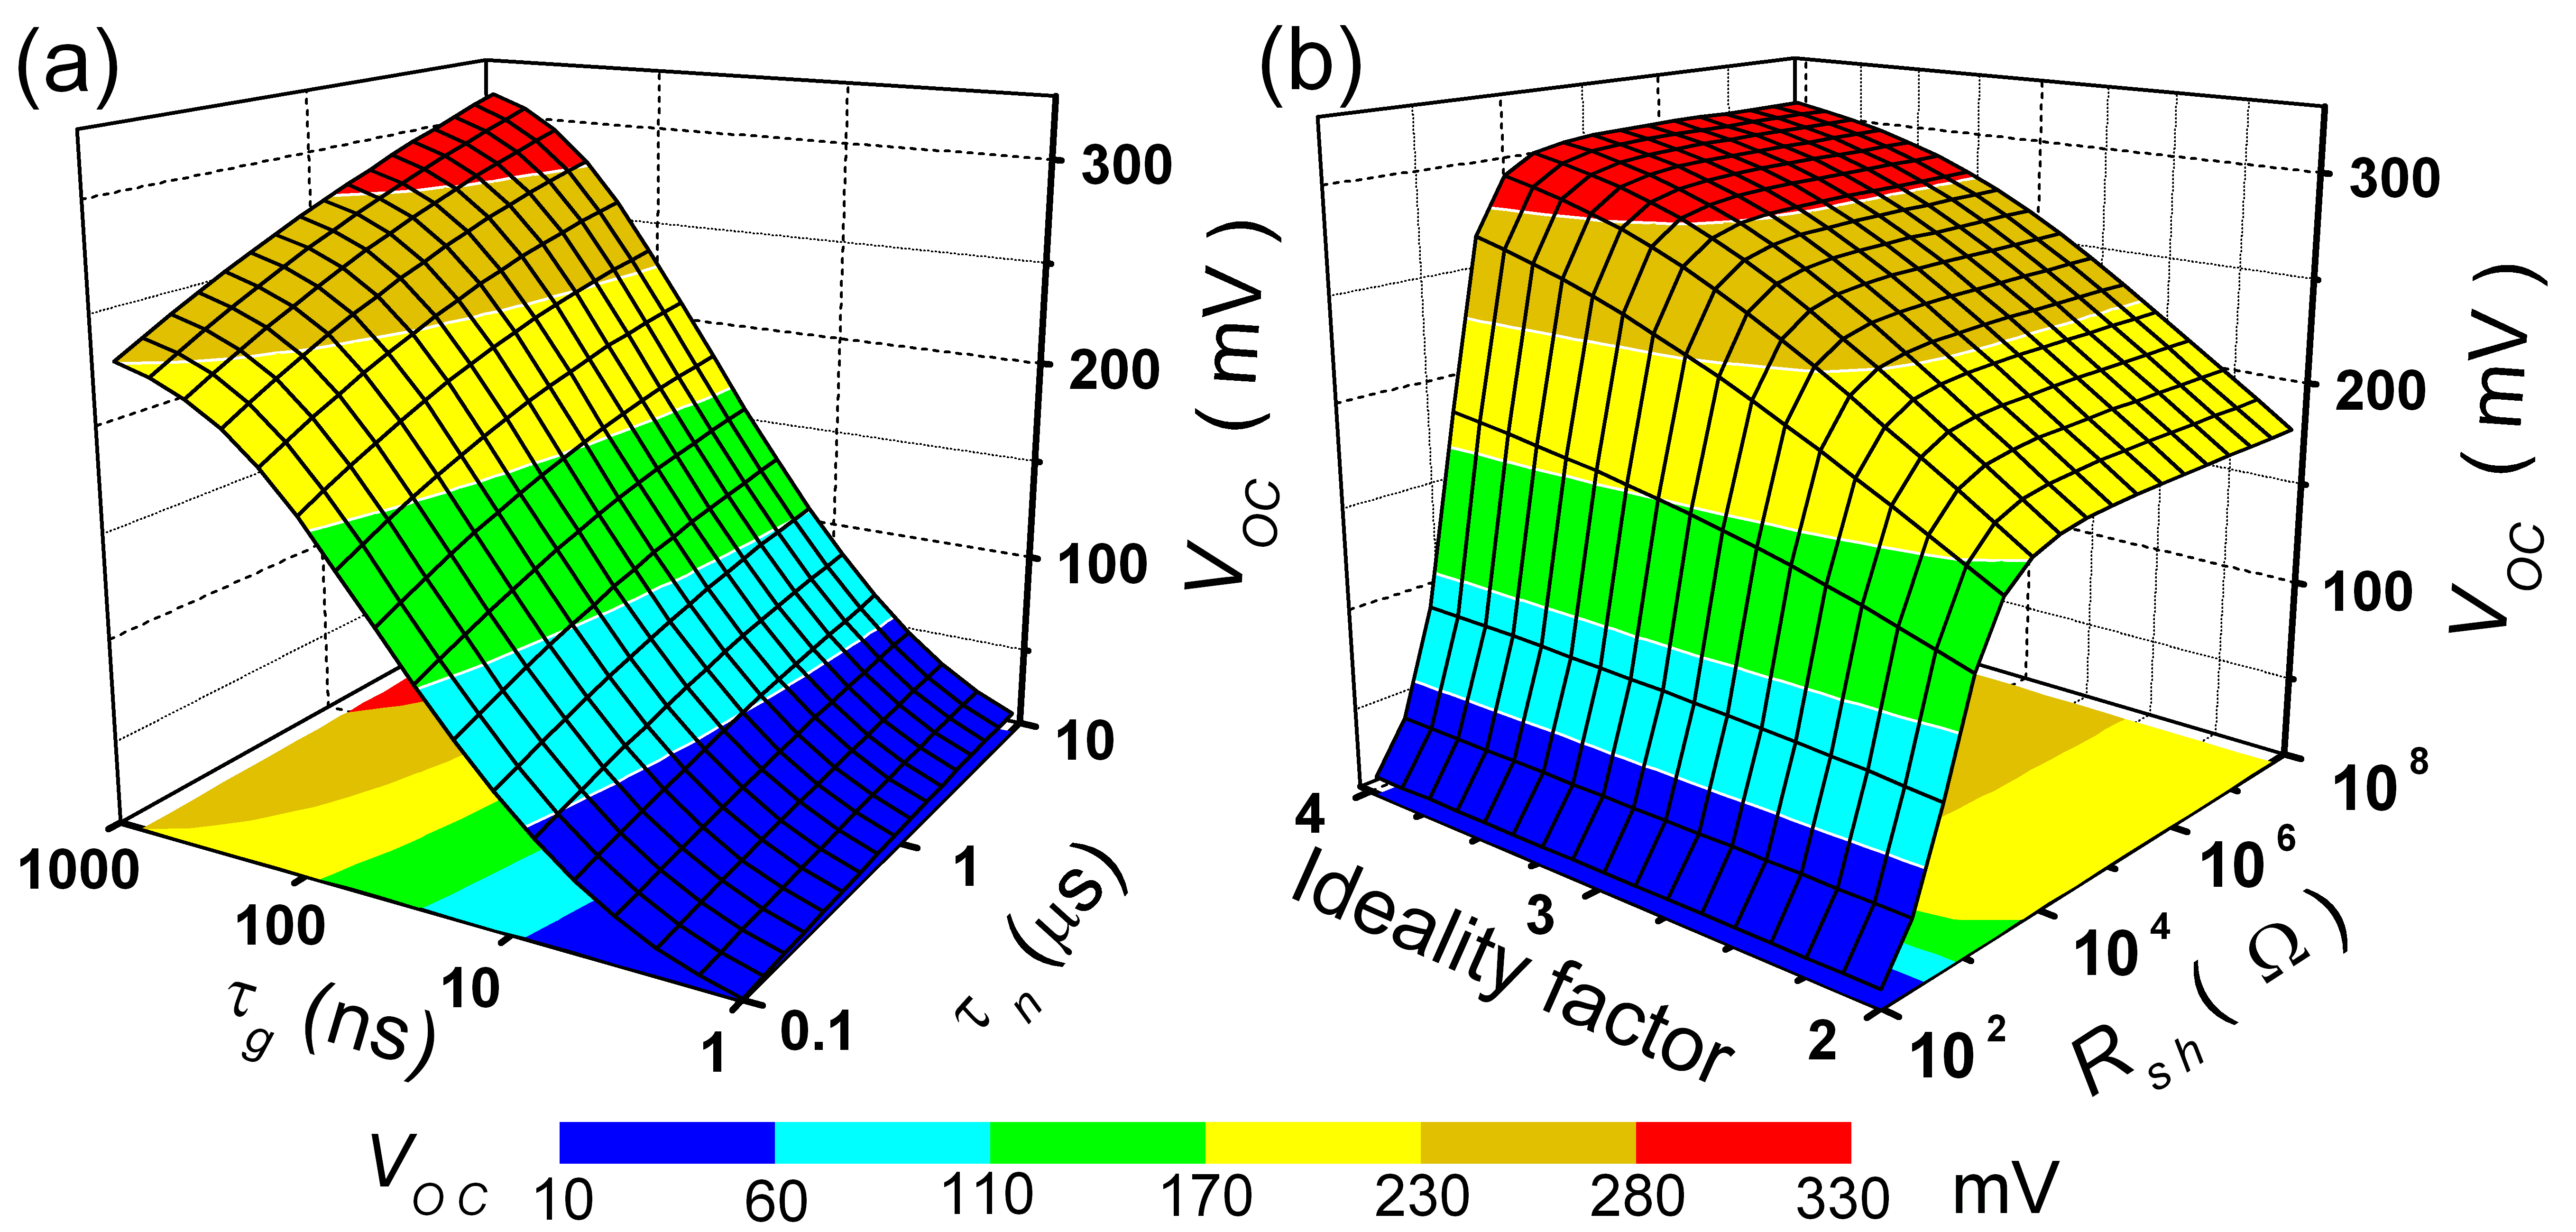
\includegraphics[width=7.5cm]{olikhFig10}%
\end{center}
\caption{\label{figDUS_Rsh}
Plot of $R_{sh}$ as the function of $kT$ for the SC--R4 with and without USL.
%$W_{U\!S}$,W/cm$^2$: 0.18 (2), 0.22 (3), 0.40 (4).
Lines are the fitted curves using Eq.~(\ref{eqRsh})
}%
\end{figure}

\Fref{figDUS_Rsh} illustrates $R_{sh}$ modification for the sample under USL condition.
One can see that the T--USL leads to moderate $R_{sh}$ decrease whereas the L--USL does not change shunt resistance practically.


Several non-mechanical reasons of SSC shunt resistance appearance are known \cite{Rsh:Breitenstein}.
They are aluminum particles, macroscopic Si$_3$N$_4$ inclusions, inversion layers at precipitates.
During firing Al will alloy in, leading to a p$^+$--doped region around the particle, which may compensate the emitter and may be in ohmic contact with the
base.
Subsequent annealing had to increase this p$^+$--region and to decrease $R_{sh}$.
Such behavior  conflicts with data, which are presented on Sec.~\ref{P3}.
Inversion layers and Si$_3$N$_4$ inclusions occur in multicrystalline silicon cells mainly \cite{Rsh:Breitenstein} and cannot cause a shunt resistance of the investigated samples too.
On the other hand, dislocations, which intersect the junction, are generally held responsible as a possible source of ohmic current \cite{Rsh:Breitenstein,TAT:Gopal,Rsh:Baker}.
Dislocations should be strongly recombinative, its recombination current may become strong enough for it to act as a shunt.
For this reason they should be decorated by impurities \cite{Rsh:Breitenstein}.

Gopal and Gupta \cite{Rsh:Gopal2003,Rsh:Gopal2004} introduced the model of dislocation--induced impedance of photovoltaic detector.
According to this model, the $R_{sh}$ can be given by
\begin{equation}
\label{eqRsh}
R_{sh}=kTR_{dis}\,\cosh\left(\frac{E_{dis}-E_i+U_s}{2kT}\right)\cosh\left(\frac{E_{dis}-E_i-U_s}{2kT}\right)\,,
\end{equation}
with
\begin{equation}
\label{eqRdis}
R_{dis}^{-1}=\rho_{dis}Aq^2A_{dis}\sqrt{K_nK_p}N_{dis}(n_p+p_p)\,,
\end{equation}
%
%\begin{eqnarray}
%\nonumber
%R_{sh}&=&\frac{kT\cosh\left(\frac{E_{dis}-E_i+U_s}{2kT}\right)\cosh\left(\frac{E_{dis}-E_i-U_s}{2kT}\right)}{\rho_{dis}Aq^2A_{dis}\sqrt{K_nK_p}N_{dis}(n_p+p_p)}\\
%\label{eqRsh}
%&=&R_{sh,0}kT\cosh\left(\frac{E_{dis}-E_i+U_s}{2kT}\right)\cosh\left(\frac{E_{dis}-E_i-U_s}{2kT}\right)\,,
%\end{eqnarray}
where
$E_{dis}$ is the energy level which significantly contributes to the dislocation recombination current,
$E_i$ is the intrinsic Fermi level,
$U_s$ is the potential at the surface of the dislocation core,
$\rho_{dis}$ and $A_{dis}$ are the dislocation density and surface area, respectively,
$K_n$ and $K_p$ are the capture probabilities for electrons and holes by the dislocation states,
$N_{dis}$ is the density of surface states at each dislocation.
Eq.~(\ref{eqRsh}) is reduced for the simplified case $K_p=K_n$.
It should be noted that a similar temperature dependence of a SSC shunt resistance is used elsewhere \cite{RshT} too.

We use Eq.~(\ref{eqRsh}) to fit the experimental $R_{sh}$ data.
$(E_{dis}-E_i)$, $U_s$ and $R_{dis}$ are taken as the fitting parameters.
It was established that the good agreement of the experimental data with the fitting curves has been observed (see \Fref{figDUS_Rsh}) for values $(E_{dis}-E_i)=(0.34\pm0.02)$~eV and $U_s=(5\pm4)\times10^{-8}$~eV, which were independent of USL.
The obtained value $(E_{dis}-E_i)$ corresponds to the carrier activation energy $E_a\simeq 0.5E_g-(E_{dis}-E_i)\simeq 0.22$~eV, which is comparable to the values reported by other researcher.
Thus activation energies $0.22\div0.25$~eV \cite{Edis:Evans}, $0.28$~eV \cite{Edis:Castaldini}, $0.19$~eV \cite{Edis:Omling} and $0.23$~eV \cite{Edis:Ogawa}  are associated with an impurity at the dislocation or with an intrinsic dislocstion levels.

%are in quite good agreement with
The $R_{dis}$ value decreases in the T--USL case and its relative changes $\varepsilon_{Rdis}$ are shown in Table~\ref{tab}.
On our opinion this is caused by an augmentation of  $A_{dis}$ in Eq.~(\ref{eqRdis}).
The dislocation core atom displacement  is  parallel and normal to the  current direction in the  L--USL  case and T--USL case respectively.
As the result, in the T--USL case carriers are captured by dislocation levels from enlarged volume.
It induces the effective surface area increase and the shunt resistance decrease.

\subsection{Ultrasound influence on SSC conversion parameters}
\Fref{figDUS_Isc} depicts an acoustically driven degradation of photocurrent, open--circuit voltage and the fill factor.
The relative changes of these parameters are listed in the Table~\ref{tab}.

\begin{figure}
\begin{center}
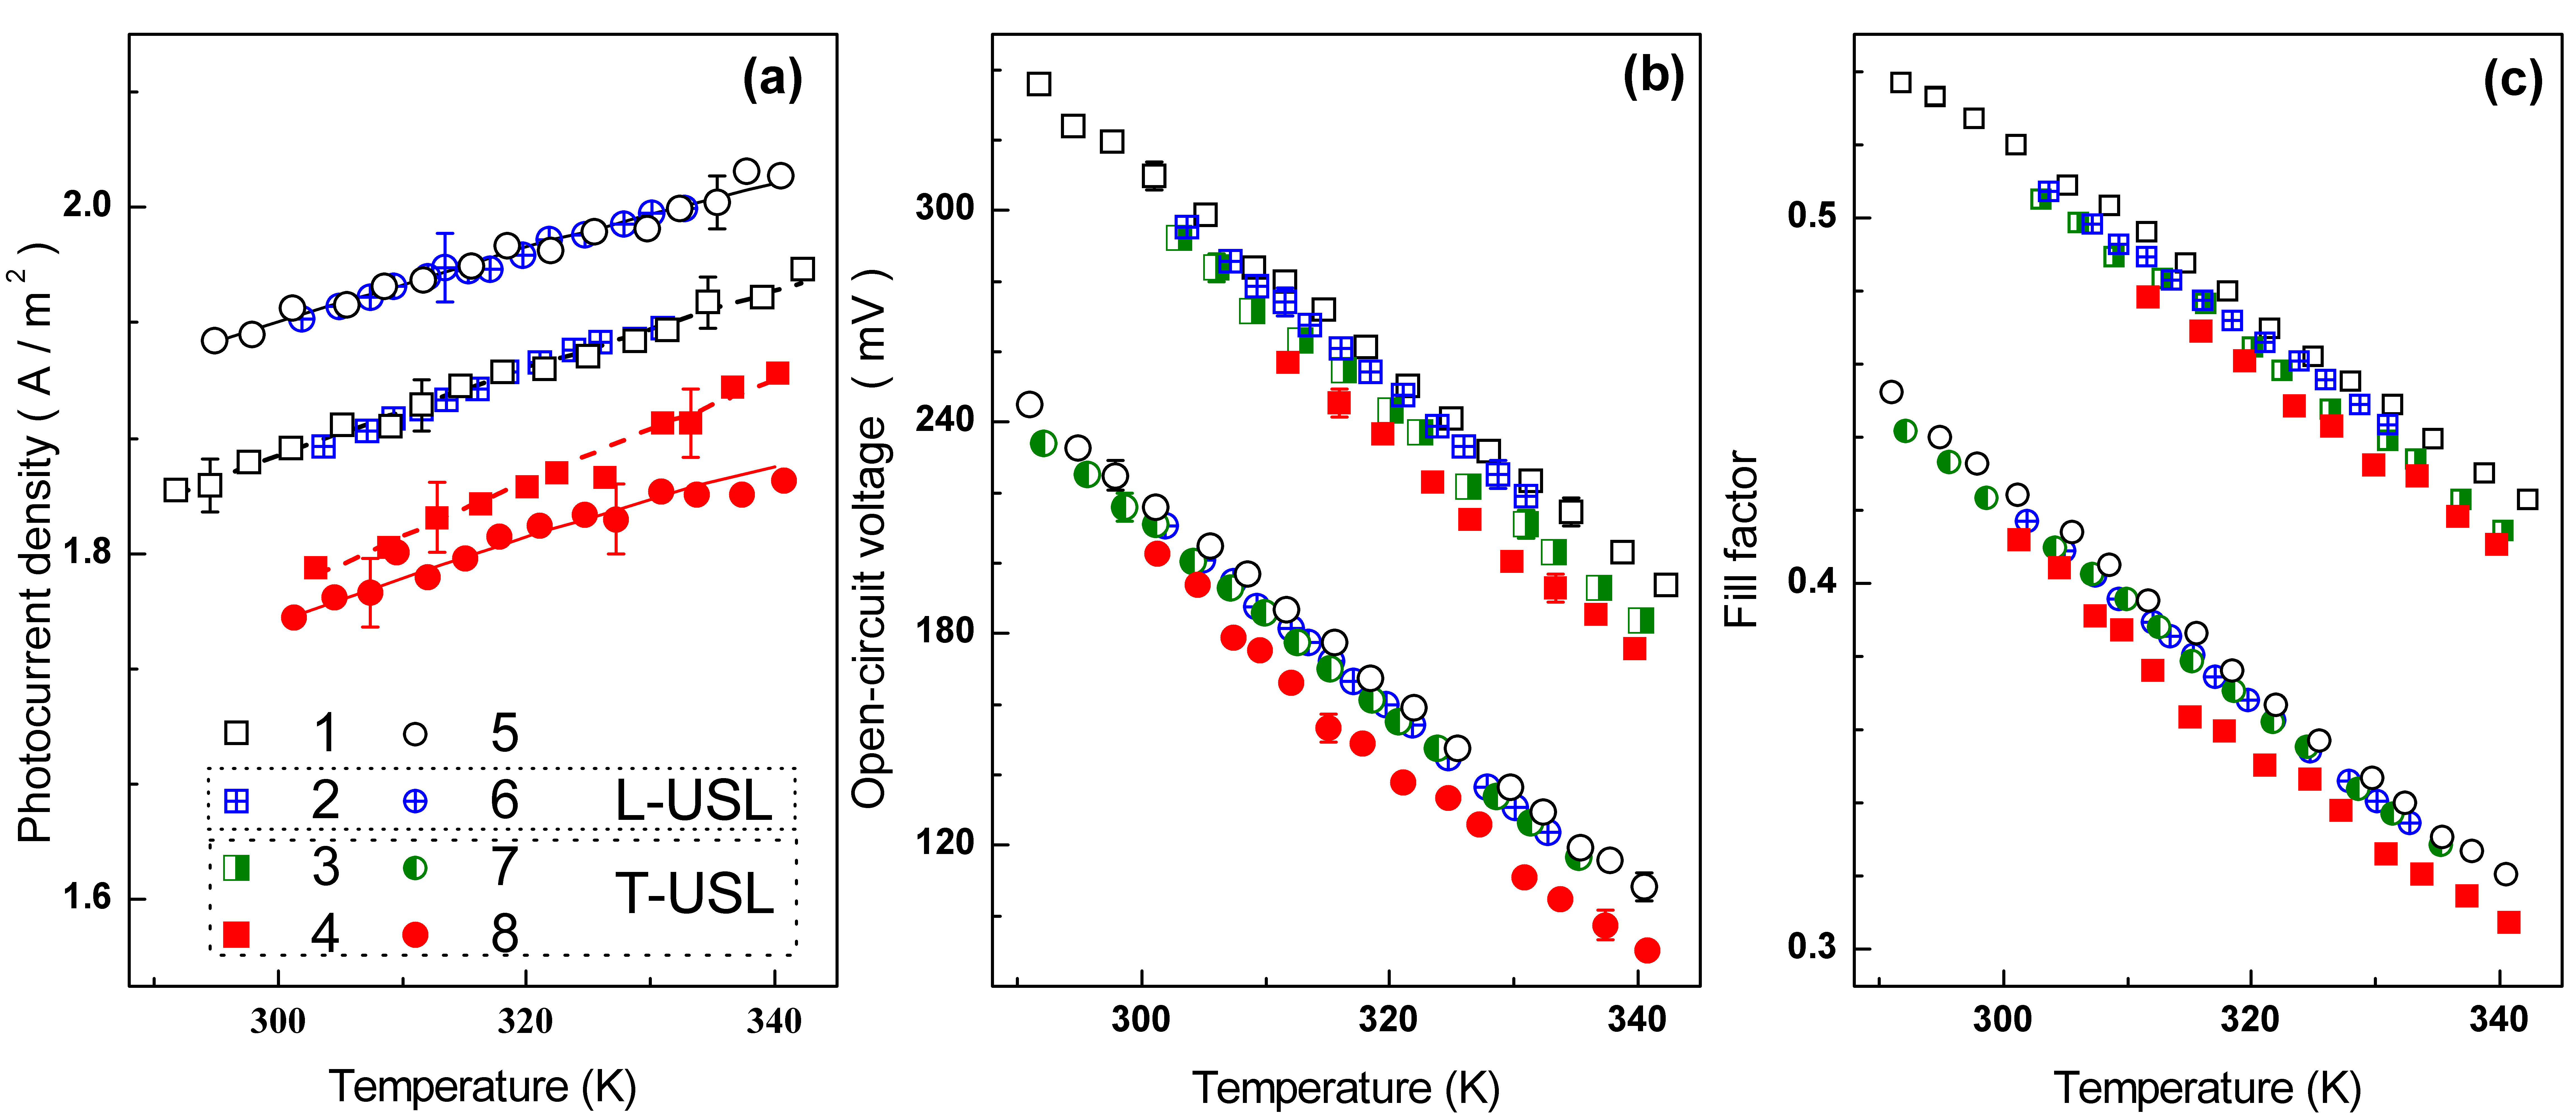
\includegraphics[width=15cm]{olikhFig11abc}%
\end{center}
\caption{\label{figDUS_Isc}
Temperature dependencies of photocurrent density (a),  open--circuit voltage (b) and  fill factor (c) for the SC--R15 (squares) and SC--R4 (circles) with (2--4 and 6--8) and without (1 and 5) USL.
$W_{U\!S}$,W/cm$^2$: 0.18 (2, 6), 0.19 (3), 0.22 (7), 0.40 (4, 8).
Lines are the fitted curves using Eq.~(\ref{eqIph}).
}%
\end{figure}

In the case of used illumination  wavelength of $\lambda=900$~nm, the photocurrent defined  by the electron�-hole pair generation in the $p$--region mainly.
If the base is several minority carrier diffusion lengths $L_n=\sqrt{\mu_nkT\tau_n/q}$, the $J_{ph}$ can be written as \cite{Markvart,Razeghi}
\begin{equation}
\label{eqIph}
J_{ph} = \frac{W_{ph}(1-M)q\beta\lambda}{hc}\frac{\alpha L_n}{1+ \alpha L_n}\,,
\end{equation}
where $\alpha$ is the absorption coefficient,
$M$ is the reflection coefficient,
$\beta$ is the coefficient of quantum yield.
Thereby $J_{ph}$ strongly depends on $\tau_n$.
On the other hand, the minority carrier lifetime can be estimated from a photocurrent temperature dependence.
We tool $\alpha$ temperature dependence from \cite{Markvart} (p.39, Eq.~(18)), and supposed, that $\beta$ and $M$ were temperature independent, $L_n\sim T^{0.5}$.
The last dependence was obtained from \Fref{figDUS_Tau}.
Then Eq.~(\ref{eqIph}) was used by taking $L_n$ as fitting parameter to fit the experimental temperature dependence of $J_{ph}$.
The fitting results are shown on  \Fref{figDUS_Isc}(a) by curves.

The $L_n$ values, which are obtained from a recombination current in the quasi-neutral region ($106\pm10$~$\mu$m and $88\pm10$~$\mu$m for SC--R4 and SC--R15 respectively at 320~K without USL) and from a photocurrent temperature dependence ($125\pm15$~$\mu$m and $99\pm15$~$\mu$m for SC--R4 and SC--R15), are comparable.
The relative changes of lifetime, obtained from $J_{ph}$,  $\varepsilon_{\tau n}^{Jph}$ are listed in the Table~\ref{tab}.
The values of $\varepsilon_{\tau n}^{Jph}$ and $\varepsilon_{\tau n}$ agree qualitatively.
The slight quantitative difference, which is observed in the T--USL case, can be deals with the AI change of $L_n$ temperature dependence probably.
Thus the ultrasound influence on photocurrent (and short-circuit current) is due to AI change of minority carrier lifetime, which is discussed above.

Unfortunately the analytical expressions for $V_{oc}$ and $FF$ are absent in the double--diode model case.
To show $V_{oc}$ and $FF$ dependencies on $\tau_n$, $n$, $\tau_g$, and $R_{sh}$ we have simulated $I$--$V$ characteristics at different parameters value by using Eqs.~(\ref{eqIV}) and (\ref{eqIph}).
The values, that are close to investigated SSCs parameters, are used for simulation.
The results are shown on \Fref{figVoc} and \Fref{figFF}.


\begin{figure}
\begin{center}

\includegraphics[width=15cm]{olikhFig12ab}%
\end{center}
\caption{\label{figVoc}
Simulated open--circuit voltage dependencies on SCR carrier lifetime and base  carrier lifetime (a) and on ideality factor and shunt resistance (b).
The constant values $n=2.55$ (a), $R_{sh}=5\cdot10^3$~$\Omega$ (a), $\tau_n=3\cdot10^{-6}$~s (b), $\tau_g=5\cdot10^{-8}$~s (b), and $T=320$~K were used.
}%
\end{figure}


\begin{figure}
\begin{center}
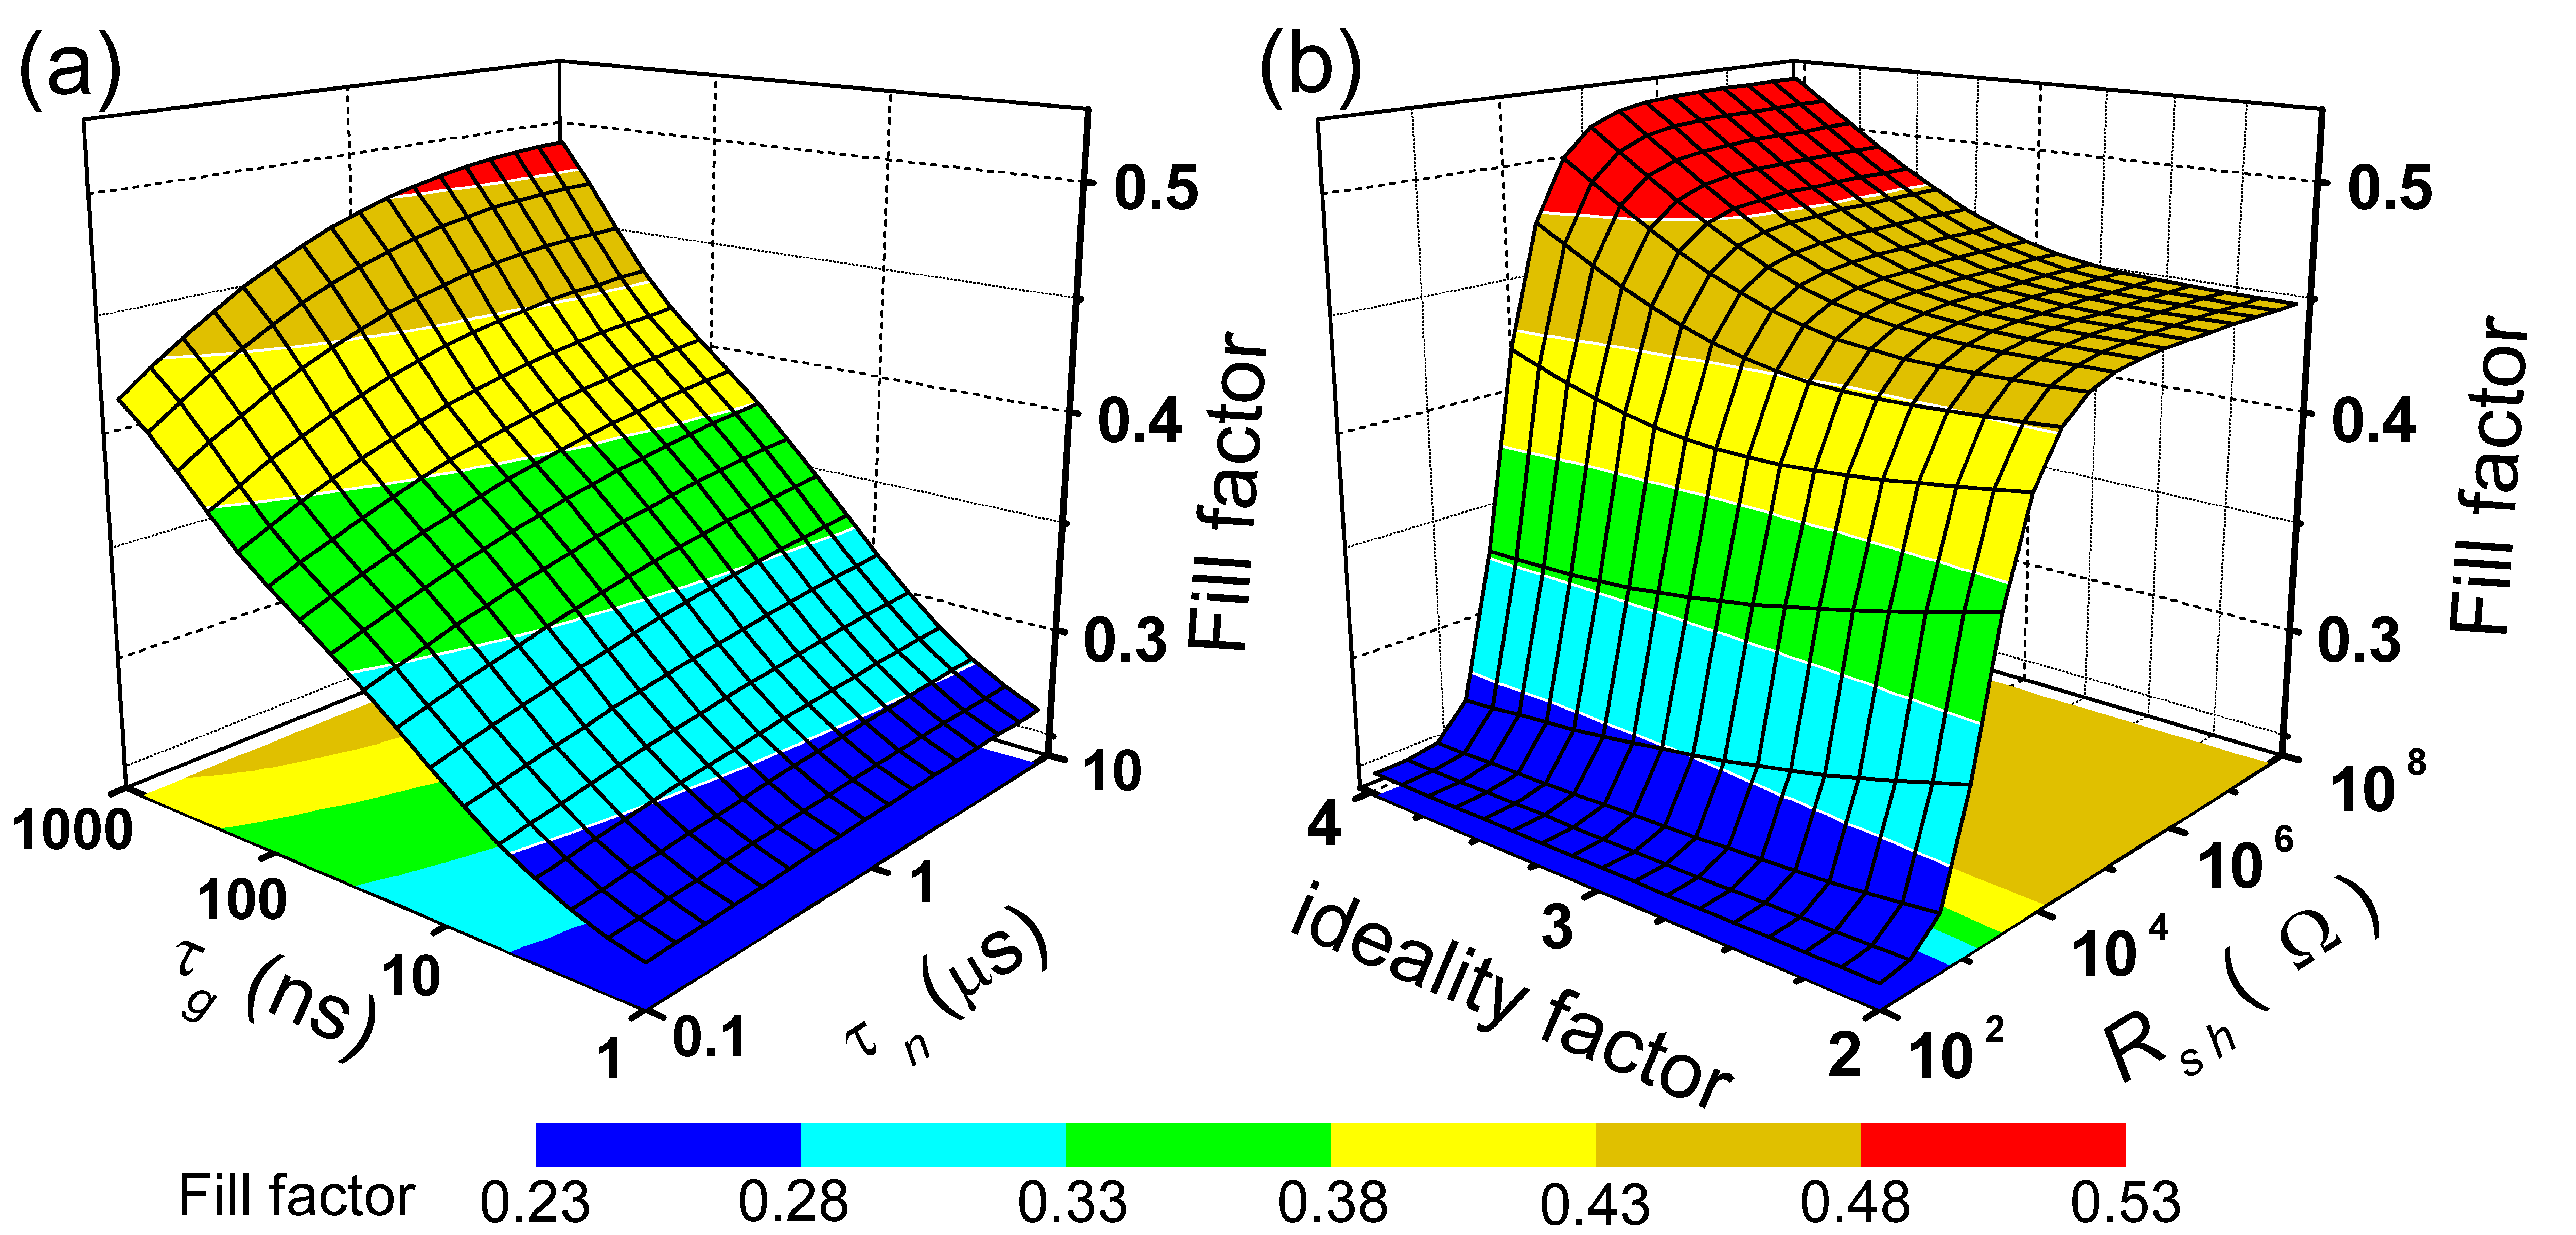
\includegraphics[width=15cm]{olikhFig13ab}%
\end{center}
\caption{\label{figFF}
Simulated fill factor dependencies on SCR carrier lifetime and base  carrier lifetime (a) and on ideality factor and shunt resistance (b).
The constant values $n=2.55$ (a), $R_{sh}=5\cdot10^3$~$\Omega$ (a), $\tau_n=3\cdot10^{-6}$~s (b), $\tau_g=5\cdot10^{-8}$~s (b), and $T=320$~K were used.
}%
\end{figure}

One can see on \Fref{figVoc}(a) and \Fref{figFF}(a) that $\tau_g$ decrease should lead to a decrement of both $V_{oc}$ and $FF$.
At the same time the open--circuit voltage and the fill factor dependencies on $\tau_n$ are weak for the investigated SSC.
\Fref{figVoc}(b) and \Fref{figFF}(b) show that the $n$ as well as $R_{sh}$ influence on $V_{oc}$ and $FF$ depends substantially on shunt resistance value.
Thus if $R_{sh}>10^5$~$\Omega$ (SC--R15 case) then $V_{oc}$ increases with an ideality factor increment and both $V_{oc}$ and $FF$ don't depend on shunt resistance value practically.
Whereas if $R_{sh}\leq10^4$~$\Omega$ (SC--R4 case) then  the open--circuit voltage and the fill factor decrease with shunt resistance decrement, but $FF$ only depends on $n$ weakly.

Thereby the discussed above AI decrease of $\tau_g$ leads to degradation of open--circuit voltage and the fill factor in the USL case.
This effect is enhanced by AI $R_{sh}$ decrease in the SC--R4 and is recovered partially by AI $n$ increase in the SC--R15.




\section{Conclusion}
The experimental investigation of ultrasound influence on the silicon solar cell has been carried out in the temperature range from 290 to 340~K.
The investigation has revealed the acoustically driven reversible degradation of SSC parameters.
It has been found out that the transverse ultrasound waves are more effective tools to affect silicon structure parameters than longitudinal ones.
It has been given evidence that the degradation is due to the recombination amplification under the ultrasound wave action.
The analysis has shown that the acoustically induced increase of carrier capture coefficient of point or extended defects is a reason of observed effects.
The qualitative model of ultrasound influence, which is based on a change of a distance between defects or between components of defect complex under alternating deformation action, is proposed.
It has been shown that the oxide precipitates are most likely defects, which take part in the acousto--defect interaction.
Thus, ultrasound can be an effective tool for controlling silicon structure characteristics.

\section*{References}
%\bibliographystyle{JoS}
\bibliography{olikh}

\end{document}

